\documentclass[
BCOR 0.7cm,							% Bindekorrektur, bspw. 1 cm
11pt										% Schriftgroesse
]{scrbook}


\newif\ifpdf
\ifx\pdfoutput\undefined
	\pdffalse              	%normales LaTeX wird ausgef�hrt
\else
	\pdfoutput=1           
	\pdftrue               	%pdfLaTeX wird ausgef�hrt
\fi

\ifpdf
	%\usepackage{ae}        % Benutzen Sie nur
	%\usepackage{zefonts}  	% eines dieser Pakete
\else
	%%Normales LaTeX - keine speziellen Fontpackages notwendig
\fi

\ifpdf %%Einbindung von Grafiken mittels \includegraphics{datei}
	\usepackage[pdftex]{graphicx} %%Grafiken in pdfLaTeX
\else
	\usepackage[dvips]{graphicx} %%Grafiken und normales LaTeX
\fi


\ifpdf
	\pdfinfo
	{
    /Author (Manfred Kindl)                                
    /Title (CIS)     
    /Subject (CIS - Handbuch)                                    
    /Keywords (CIS FH-Complete)	
  }
\else			
\fi

\usepackage{listings} \lstset{numbers=left, numberstyle=\tiny, numbersep=5pt}
\lstset{language=tex} 


\usepackage[pdftex,colorlinks=true,urlcolor=blue,linkcolor=blue]{hyperref}
\usepackage[ngerman]{babel}		%Deutsche Worttrennung	
\usepackage[T1]{fontenc}    % T1-Kodierung damit Umlaute richtig dargestellt werden
\usepackage[left]{eurosym}   %Paket f�rs Eurosymbol
\usepackage[latin9]{inputenc} % latin9 Encoding
\usepackage{makeidx} % Stichwortverzeichnis erstellen aus \index{} Eintr�gen
\usepackage{float}
\usepackage[small,bf]{caption}
\usepackage{fancyhdr} % Paket zur Manipulation von Kopf und Fusszeile
\usepackage{amssymb,amsmath}
\usepackage{color}
\usepackage{hyperref} % Paket zum formatieren der Hyperlinks
\hypersetup{colorlinks=false} % Formatiert die internen Links nicht. Optionen siehe unter: http://en.wikibooks.org/wiki/LaTeX/Hyperlinks#Customization

\addtokomafont{chapter}{\color[rgb]{0.0,0.376,0.584}} %Schriftfarbe f�r Kapitel�berschriften
\addtokomafont{section}{\color[rgb]{0.0,0.376,0.584}} %Schriftfarbe f�r Kapitel�berschriften
\addtokomafont{subsection}{\color[rgb]{0.0,0.376,0.584}} %Schriftfarbe f�r Kapitel�berschriften


\renewcommand{\rmdefault}{phv} % Arial
\renewcommand{\sfdefault}{phv} % Arial


\makeindex

\graphicspath{{../../../images/}}

\setlength{\tolerance}{2000}
\setlength{\parindent}{0pt}
\setlength{\parskip}{1ex plus 0.5ex minus 0.2ex}
\addtolength{\textheight}{2cm}
\addtolength{\headheight}{2pt}
\setlength{\captionmargin}{20pt}
\floatstyle{plain}
\floatname{example}{Example}

\newfloat{example}{hbtp}{loe}[chapter]
\floatplacement{figure}{hbtp}
\floatplacement{table}{htbp}

\newcommand{\dollar}{\char36}
\renewcommand{\labelitemi}{
\includegraphics[width=5pt]{blacksquare}}
\renewcommand{\labelitemii}{--}
%\renewcommand*{\chapterformat}{\textcolor{red}}

\newenvironment{info}[1]{
    %\hspace{-10mm}
     \framebox[\textwidth][l]{
        \begin{minipage}{1,3cm}
        
\includegraphics[width=1cm]{icon_info}
        \end{minipage}
        \begin{minipage}{12cm}
        #1
        \end{minipage}
    }
}

\newenvironment{achtung}[1]{
    %\hspace{-10mm}
     \framebox[\textwidth][l]{
        \begin{minipage}{1,3cm}
        
\includegraphics[width=1cm]{icon_achtung}
        \end{minipage}
        \begin{minipage}{12cm}
        #1
        \end{minipage}
    }    
}

\newenvironment{halt}[1]{
    %\hspace{-10mm}
     \framebox[\textwidth][l]{
        \begin{minipage}{1,3cm}
        
\includegraphics[width=1cm]{icon_halt}
        \end{minipage}
        \begin{minipage}{12cm}
        #1
        \end{minipage}
    }
}

\newenvironment{idee}[1] {
    %\hspace{-10mm}
     \framebox[\textwidth][l]{
        \begin{minipage}{1,3cm}
        
\includegraphics[width=1cm]{icon_idee}
        \end{minipage}
        \begin{minipage}{12cm}
        #1
        \end{minipage}
    }
}


\setlength{\unitlength}{1mm}

\newenvironment{markier}[5]{
    
    \thicklines \put(#2,#3){\vector(#4,#5){5}} \thinlines
    \put(#2,#3){\circle*{5}}
    \put(#2,#3){\textcolor{black}{\circle{5}}\makebox(-10,0){\textcolor{white}{#1}}}


}


\hyphenation{gleich-zeitig para-meter}


\begin{document}

\ifpdf
	\DeclareGraphicsExtensions{.pdf,.jpg,.png}
\else
	\DeclareGraphicsExtensions{.eps}
\fi

\pagestyle{fancyplain}

%% Titelseite einbinden %%%%%%%%%%%%%%%%%%%%%%%%%%%%%%%%%%%%%%%%%%%%%

%
% Titelseite, Abstrakt, Danksagung und Inhaltsverzeichnis
%
%% eigene Titelseitengestaltung %%%%%%%%%%%%%%%%%%%%%%%%%%%%%%%%%%%%%%%    

\begin{titlepage}
\begin{center}

\vfill 
\includegraphics[width=1\textwidth]{fhcomplete}\vspace*{20mm}
\vfill 
\includegraphics[width=100mm]{cis}
\vspace*{10mm} 

\huge Handbuch\\

	
\large \vfill FH Technikum Wien\\

Wien, \today
\end{center}
\end{titlepage}

\tableofcontents			% Inhaltsverzeichnis
\frontmatter					% Vorspann (z.B. r�mische Seitenzahlen)
%\chapter{Einleitung}
%\info{Alle im Handbuch gezeigten Abbildungen wurden mit Daten aus der Entwicklungsdatenbank zur besseren Veranschaulichung der Abl�ufe erzeugt. Die Inhalte der Listen, wie etwa Betr�ge oder Zugriffsrechte, sind frei erfunden und haben keinen Bezug zu den Daten des Echtsystems.}
\mainmatter						% Hauptteil

%% Kapitel Anfang %%%%%%%%%%%%%%%%%%%%%%%%%%%%%%%%%%%%%%%%%%%%%%%%%

\chapter{Begriffserkl�rung, Features und verwendete Abk�rzungen}
\label{Kapitel Begriffe}

	\minisec{Einheit}
...siehe Lehreinheit.
	
	\minisec{Fachbereich}
...siehe Institut.

	\minisec{Institut}
Ein Institut ist die zust�ndige Stelle f�r die Vergabe von Lektoren an die einzelnen Studieng�nge und Lehrf�cher.
Ein Beispiel ist das Institut ''Sprachen'', der f�r alle sprachbezogenen Lehrf�cher zust�ndig ist. (Englisch, Franz�sisch, Japanisch,...)

	\minisec{Kollision}
TEMPUS\raisebox{1ex}{\tiny \copyright} 2.0 �berpr�ft bei Eintragungen und Verschiebungen im LV-Plan die Verf�gbarkeit von Lektoren, Studenten und R�umen, sowie Zeitsperren der Lektoren und Reservierungen. Sollte es zu einer Terminkollision mit einem der drei Pl�ne kommen, erscheint eine Fehlermeldung und die Aktion wird abgebrochen.
Durch Deaktivieren der Kollisions�berpr�fung im Men�punkt ''Einstellungen'' kann jedoch eine Kollision erzwungen werden. Dies sollte jedoch stets nach Gebrauch wieder deaktiviert werden, da es sonst leicht zu Fehlplanungen kommen kann. (siehe Kapitel \ref{Kapitel Kollisionen})

	\minisec{KW...Kalenderwoche}
Das Jahr umfasst mindestens 52 durchnummerierte Kalenderwochen (KW). Die erste Woche des Jahres nach DIN 1355 / ISO 8601 ist die erste Woche, in die mindestens vier Tage des neuen Jahres fallen. 

	\minisec{Kollegium}
Das Kollegium setzt sich aus allen StudiengangsleiterInnen sowie VertreterInnen der Lehrenden, FachbereichsleiterInnen und StudentInnen zusammen und trifft wichtige strategische Entscheidungen f�r die Fachhochschule Technikum Wien.
	
	\minisec{LE...Lehreinheit}
In der Lehreinheit verschmelzen die wesentlichen, ver�nderlichen Daten um mit der Planung fortfahren zu k�nnen. Die Daten in den Lehreinheiten dienen speziell f�r die LV-Planung und auch als Datenquelle f�r die CIS-Seite. Lehrauftr�ge werden auch auf Basis dieser Daten erstellt. 

Die Lehreinheit f�hrt Lektoren, Studenten, Lehrf�cher usw. zusammen und muss jedes Semester �berarbeitet werden.

Eine detailierte Beschreibung finden Sie in Kapitel \ref{Kapitel Lehreinheiten}

Siehe zum Vergleich ''LV...Lehrveranstaltung''

	\minisec{Lehreinheit\_ID}
Die Lehreinheit\_ID ist eine interne Nummer, die vom System eindeutig jeder Lehreinheit zugeteilt wird.
Die meisten Tabellen der Datenbank sind mit der Lehreinheit\_ID verkn�pft

	\minisec{Lehrfach}
Ein Lehrfach bestimmt den Inhalt einer Lehreinheit. (z.B. Mathematik)

In ihr definiert sind der verantwortliche Fachbereich, die Farbe (die im Stundenplan angezeigt wird) und die Unterrichtssprache. Ein Lehrfach wird f�r jeden Studiengang und jedes dazugeh�rige Semester angelegt. Die Kurzbezeichnung des Lehrfachs wird gemeinsam mit der Lehrform an erster Stelle im Lehrveranstaltungsplan angezeigt. 
Die Lehrform des Unterrichts (�bung, Vorlesung, ILV, ...) wird hier jedoch nicht bestimmt.

	\minisec{Lehrform}
Die Lehrform beschreibt das Lehrfach detaillierter, indem sie angibt, in welchem Stil der Unterricht stattfindet. 

Eine Lehrform kann Beispielsweise die Vorlesung (-VO) sein. Dies beschreibt einen Frontalunterricht ohne selbstst�ndige �bungen. 

Andere Beispiele sind �bung (-UE), Integrative Lehrveranstaltung (-ILV), Laborstunden (-LAB) oder Tutorien (-TUT)

	\minisec{Lehrveranstaltungsplan (=Stundenplan)}
Der Lehrveranstaltungsplan (kurz ''LV-Plan'') ist die Oberfl�che auf der graphisch die Lehreinheiten mit den unterrichtenden Lektoren, dem Lehrverband und dem Raum farblich dargestellt werden. 

Am LV-Plan kann durch die R�ume und die Unterrichtswochen gebl�ttert werden und der LV-Plan kann dort auch f�r diverse andere Anwendungen exportiert werden.

	\minisec{Lehrverband}
Der Lehrverband bezeichnet die Gliederung der Studenten in Studiengang, Semester, Verb�nde und Gruppen. 

Er dient der Schlichtung und Aufteilung gr��erer Studentenzahlen um kleinere und �bersichtlichere Gruppen zu schaffen. 

Ein Beispiel an der FH Technikum-Wien w�re: BEL-2A1. (Studiengang Bachelor Elektronik, 2. Semester, Verband A, Gruppe 1) 

	\minisec{LFVT...Lehrf�cherverteilung}
Die Lehrf�cherverteilung ist die gesamte Liste aller Lehreinheiten, die in einem Semester eines Studienganges zu verplanen sind.

	\minisec{LV...Lehrveranstaltung}
Als Lehrveranstaltung wird im Gesamtsystem das gleiche verstanden, wie im Antrag des Studiengangs. In ihr enthalten sind die grundlegenden Stammdaten. Im Gegensatz zu der Lehreinheit enth�lt die Lehrveranstaltung Daten, die im Wesentlichen von Jahr zu Jahr unver�ndert bleiben. Sie bildet das Grundger�st auf dem alle anderen Tabellen aufbauen.\\
Die Lehrveranstaltung wird immer aus Sicht eines Studiengangs oder aus der Sicht des Studenten gesehen. Der Titel der Lehrveranstaltung findet sich im Zeugnis und im Lehre-Bereich im CIS wieder. Nicht zu verwechseln ist die Lehrveranstaltung mit dem Lehrfach oder der Lehreinheit (siehe eigene Begriffserkl�rungen).\\
Einmal verwendete Lehrveranstaltungen k�nnen nicht mehr entfernt sondern nur deaktiviert werden, da Notenzuordnungen verloren gehen w�rden.

Attribute der Lehrveranstaltung sind beispielsweise die Kurzbezeichnung, der Studiengang, das Semester in dem diese unterrichtet wird, die Sprache, die ECTS-Punkte oder die Semesterstunden.

	\minisec{Module, Spezialgruppen}
Neben den regul�ren Lehrverbandsgruppen gibt es Module und Spezialgruppen, die unterschiedliche Studenten beherbergen k�nnen.
Es ist damit m�glich, Studenten aus verschiedenen Lehrverbandsgruppen innerhalb eines Semesters aber auch semester- und studiengangs�bergreifend zusammenzufassen. Da eine Kollisionspr�fung und korrekte Verplanung durch Spezialgruppen aber erheblich erschwert wird, sollten Spezialgruppen m�glichst vermieden werden.

	\minisec{Quickinfo}
Eine Quickinfo erscheint, wenn der Mauszeiger l�ngere Zeit ohne zu klicken �ber einem Element steht.

	\minisec{Raumtyp}
Um die verschiedenen Unterrichtsr�ume zusammenzufassen, wird das Attribut ''Raumtyp'' verwendet.
Ein Raumtyp w�re beispielsweise ''Seminarraum''. Dieser fasst beliebig viele, einzelne R�ume zu einer Gesamtheit zusammen.
Das Attribut dient haupts�chlich dazu, um bei der Stundenverplanung eine �bersichtliche Menge an Raumvorschl�gen f�r eine Lehreinheit zu erhalten.

	\minisec{Reservierung}
Der Lehrveranstaltungsplan bietet Lektoren und Angestellten die M�glichkeit der Reservierung, um sich mittelfristig einen Raum zu sichern und f�r die Lehrveranstaltungsplanung und andere Mitarbeiter zu sperren.
Die Reservierung eines Raumes ist in einem vordefinierten Zeitfenster m�glich. Eine get�tigte Reservierung hat normalerweise Vorrang vor dem regul�ren Unterricht.

Dies stellt sich in der Praxis aber als �u�erst hinderlich dar. Oft sind externe Veranstaltungen, Gastvortr�ge, Feiern und Sponsionen ein Grund f�r unangenehme Verschiebungen und Raumzuteilungen. Jene irregul�ren Veranstaltungen sind aber ein wichtiger Teil des Fachhochschulbetriebs und so wird sich vermutlich keine angenehmere L�sung finden lassen, als solchen Veranstaltungen Vorrang zu geben.

	\minisec{Semester (Jahrgang)}
Ein Semester (von lat.: sex=sechs; mensis=Monat) ist ein Studienhalbjahr an einer Hochschule. Dabei sind die Semesterferien (=vorlesungsfreie Zeit) einbezogen.
F�r gew�hnlich sind ungerade Semester (1,3,5,...) im Wintersemester (von September bis Februar) und gerade Semester (2,4,6,...) im Sommersemester (von M�rz bis August) 

	\minisec{Spezialgruppen}
...siehe Module

	\minisec{Studiengang}
Ein Studiengang ist ein, hinsichtlich eines Studienabschlusses eines wissenschaftlichen Studienfaches, angebotener Lerninhalt an einer Hochschule. 

Das Curriculum eines Studienganges wird durch die Studienordnung, die Pr�fungsleistungen und den Abschluss durch die Pr�fungsordnung definiert. 

Ein Studiengang schlie�t mit einem akademischen Grad zum Beispiel Diplom, Bachelor oder Master ab.

	\minisec{Studiensemester}
Das Studiensemester ist eine eindeutige Zuordnung zu einem Semester und einem Kalenderjahr.
Demnach ist ''WS2007'' das Wintersemester im Jahr 2007.

	\minisec{Stundenblockung}
Die Stundenblockung gibt an, wie viele Einheiten am St�ck (also direkt hintereinander) verplant werden sollen. Da (bei Einheiten zu 45 Minuten) eine Einzelstunde oft unzureichend ist, wird die Stundenblockung in den meisten F�llen zumindest ''2'' betragen.

	\minisec{Stundenplan}
...siehe Lehrveranstaltungsplan

	\minisec{UNR...Unterrichtsnummer}
Die Unterrichtnummer ist eine fortlaufende Zahl, die vom System automatisch generiert wird und haupts�chlich f�r Abl�ufe im Hintergrund relevant ist. Normalerweise wird die UNR gleichgesetzt mit der Lehreinheit\_ID. 
Wichtig zu wissen ist, dass die Kollisions�berpr�fung des LV-Plans anhand der UNR erfolgt. Lehreinheiten mit der gleichen UNR k�nnen also parallel verplant werden, ohne dass eine Fehlermeldung erfolgt.

	\minisec{Unterrichtseinheit}
Ein Tag kann in beliebig viele Unterrichtseinheiten mit einer Beginn- und Endzeit aufgeteilt werden. Dabei d�rfen sich allerdings die Beginnzeiten nicht �berschneiden.
Am Beispiel Technikum-Wien erfolgt die Unterteilung in 16 Einheiten zu je 45 Minuten, beginnend mit 08:00 Uhr.

	\minisec{Wochenrhythmus}
Wird eine Lehrveranstaltung in regelm��igen Abst�nden �ber das Semester verteilt, kann beim Attribut ''Wochenrhythmus'' das Intervall angegeben werden.
Ein Wochenrhythmus ''2'' bedeutet demnach, dass die LV alle 2 Wochen stattfinden soll.

	\minisec{Zeitsperre}
Die Zeitsperre ist eine Erweiterung des Features ''Zeitwunsch'', um detailliertere Informationen zur Verf�gbarkeit eines Lektors zu bekommen.
Der/DIe LektorIn erh�lt dadurch die M�glichkeit, unbegrenzt viele Termine punktuell zu sperren (Beispielsweise wegen Konferenzen, Auslandsaufenthalten, Urlaub oder Schulungen). Eine Zeitsperre wird im LV-Plan dunkelrot hervorgehoben und erzeugt beim verplanen eine Kollision. (siehe Kapitel \ref{Kapitel Kollisionen})

	\minisec{Zeitwunsch}
Jedem/Jeder LektorIn wird in seinem Profil die M�glichkeit gegeben, Zeitpr�ferenzen f�r seinen Unterricht anhand eines Normwochenrasters einzutragen. Der Lektor kann f�r jeden Tag und jede Unterrichtseinheit einer Woche Gewichtungen von -2 bis +2 geben um so seine Verf�gbarkeit anzugeben. Dieses Muster wird dann f�r alle Wochen eines Semesters �bernommen.
Die Zeitw�nsche sollen nach dem Fairplay-Prinzip gew�hlt werden, so dass mindestens doppelt so viele positiv bewertete Einheiten vorhanden sind, wie laut Lehrauftrag zu unterrichten w�ren.

\begin{tabular}{rll}
+2&...&hier m�chte ich unterrichten\\
+1&...&hier kann ich unterrichten\\
-1&...&hier nur in Notf�llen\\
-2&...&hier kann ich gar nicht unterrichten\\
\end{tabular}

Die Werte werden durch ein Farbsystem (von Rot bis Gr�n) im Hintergrund angezeigt. Die Standardeinstellung ist +1. 

Die Praxis zeigt aber, dass Lektoren dieses Feature oft nicht in Anspruch nehmen oder derart in der Flexibilit�t eingeschr�nkt sind, dass eine reibungsfreie Planung nicht m�glich ist. In Einzelf�llen werden sogar weniger Einheiten positiv bewertet, als pro Woche zu unterrichten sind.
Au�erdem werden die Zeitw�nsche selten auf den neuesten Stand gebracht, was wiederum zu nachtr�glichen �nderungen f�hrt.
Ein disziplinierter Gebrauch der Zeitw�nsche ist also ein wesentlicher St�tzpunkt f�r eine effektive Lehrveranstaltungsplanung.

Im Programm TEMPUS\raisebox{1ex}{\tiny \copyright} wird der Zeitwunsch bei Auswahl eines Lektors oder beim setzen einer Lehreinheit durch die Hintergrundfarbe angedeutet.

\begin{figure}
	\centering
	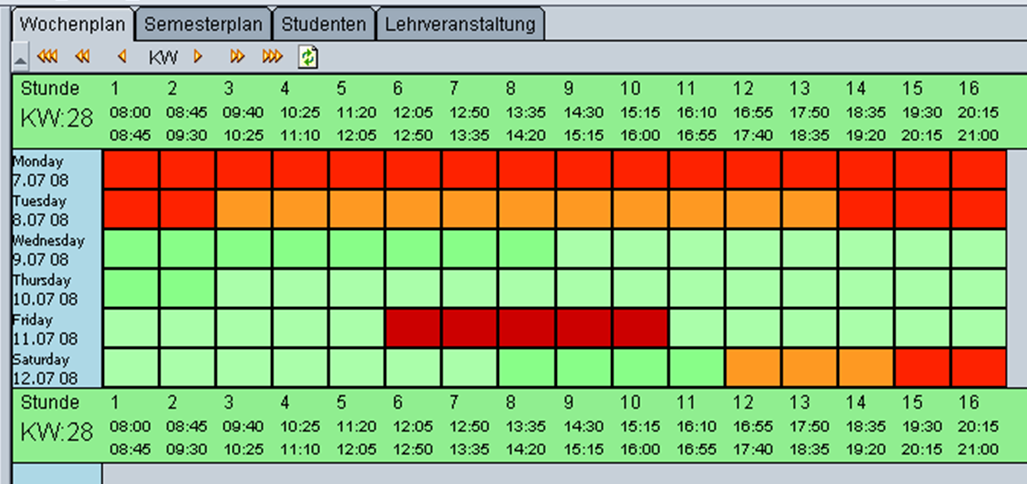
\includegraphics[width=0.8\textwidth]{Tempus_Beispiel_Zeitwunsch}
	\caption{Beispiel eines Zeitwunsches mit allen vier Werten und einer Zeitsperre (Dunkelrot) am Freitag}
	\label{Zeitwunsch}
\end{figure}
\chapter{Allgemeines}
\section{�berblick}

Das Campus Informationssystem ist die zentrale Web-Oberfl�che f�r Studierende und MitarbeiterInnen. Hier werden verschiedene Servicedienste zur Verf�gung gestellt.
Hier finden Sie News, k�nnen sich �ber die Lehre informieren, Lehrveranstaltungspl�ne abrufen und vieles mehr. 

\begin{figure}
	\centering
	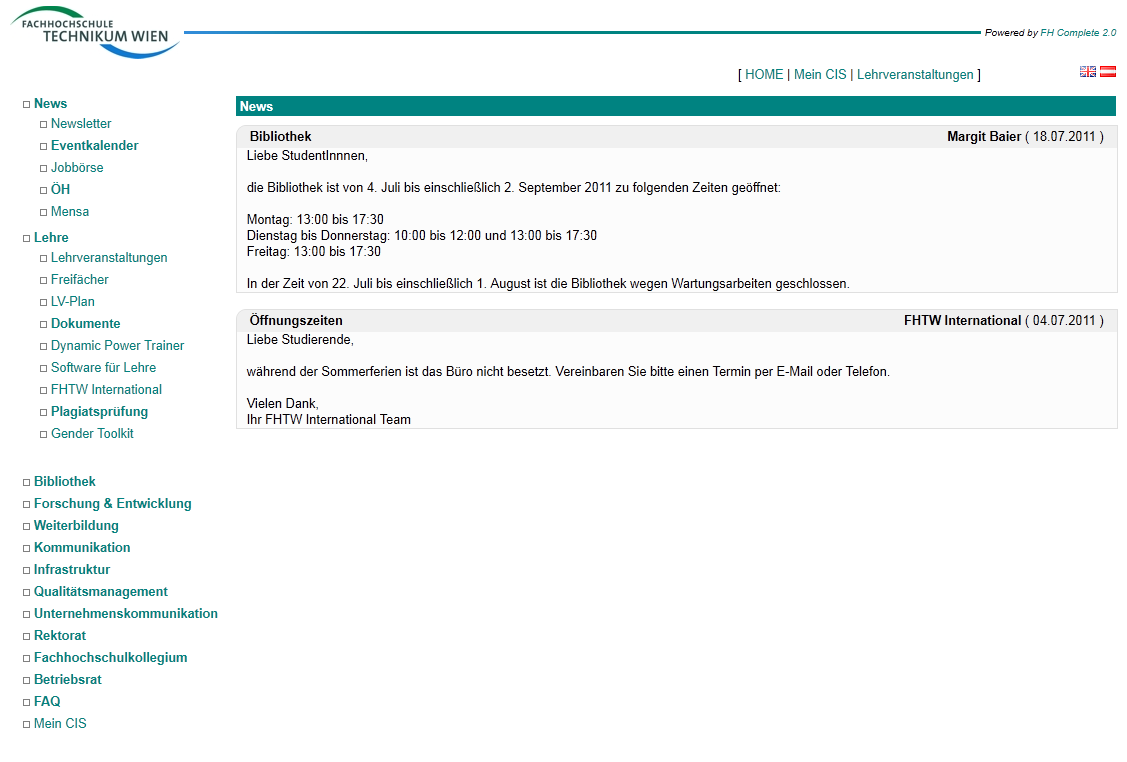
\includegraphics[width=0.70\textwidth]{CIS_Startseite.png}
	\caption{CIS Startseite}
	\label{CIS_startseite}
\end{figure}

\section{Hauptmen�punkte}

	\minisec{News}
Im CIS gibt es verschieden Ansichten f�r News (im Bereich der LV-News auch Pinboard genannt). Auf der Startseite befindet sich die Ansicht f�r "`allgemeine News"'. Des weiteren gibt es Ansichten f�r die einzelnen Organisationseinheiten (Studiengang, Institut, ...). Diese werden auf den entsprechenden Unterseiten angezeigt und dort mit den allgemeinen News gemischt.
Die Richtlinien zur Newsverwaltung entnehmen Sie bitte  Kapitel \ref{richtlinien_newseintraege}

Der Abschnitt "`News"' im CIS beinhaltet auch Links zu anderen externen News und Informationsplattformen.

	\minisec{Lehre}
Der Bereich Lehre umfasst alle notwendigen Informationen und Unterlagen zur Durchf�hrung der Lehre wie Infos zu Lehrveranstaltungen, Anwesenheitslisten, Notenlisten, TeilnehmerInnenlisten, Mailgruppen, Semesterplan und das Abgabetool zur leichteren Durchf�hrung von �bungen.

Au�erdem kann man sich in diesem Bereich f�r Freif�cher anmelden und findet Tools und Informationen zur Durchf�hrung der Lehre.
Details dazu entnehmen Sie bitte dem Kapitel \ref{lehre}.

	\minisec{Bibliothek}
Hier finden Sie Informationen zur Bibliothek, Recherche-Links, Verweise zu elektronischen Medien und externen Literaturdatenbanken sowie die Publikationsdatenbank OPUS.

	\minisec{Forschung \& Entwicklung}
Informationen zu laufenden Projekten sowie Dokumente und Prozessabl�ufe f�r die Durchf�hrung von Forschungsprojekten sind unter diesem Men�punkt zu finden.

	\minisec{Weiterbildung}
Hier k�nnen Sie sich �ber das aktuelle interne und externe Weiterbildungsprogramm informieren.

	\minisec{Kommunikation}
Hier k�nnen Kontakte, eine Personensuche, das Webmail und Mailverteiler der FHTW abgerufen werden.

	\minisec{Infrastruktur}
Im Bereich Infrastruktur sind die wichtigsten Informationen rund um die technische und logistische Infrastruktur im Haus gesammelt:
Anleitungen und Tools zur Registration im LAN und WLAN, ein kostenloses Anti-Viren Programm, Infos zur Medienausstattung, Lagepl�ne sowie Verordnungen.

	\minisec{Qualit�tsmanagement}
Hier finden Sie alle studienrelevanten Dokumente und Prozessabl�ufe und Dokumente zur allgemeinen Organisation der FHTW sowie die relevanten Dokumentvorlagen.

	\minisec{Unternehmenskommunikation}
In diesem Men�punkt stehen das Logo der FHTW, Corporate Identity Handb�cher und ein Veranstaltungsleitfaden zum Download zur Verf�gung.

	\minisec{Rektorat}
Unter "`Rektorat"' finden Sie das Leitbild der FHTW, Kennzahlen, Gender Mainstreaming-Aktivit�ten, Hochschulprojekte, Auszeichnungen sowie Infos zu Wettbewerbsausschreibungen und Stipendien.

	\minisec{Fachhochschulkollegium}
	In diesem Men�punkt sind die Zusammensetzung und Gesch�ftsordnung des Kollegiums der FH Technikum Wien sowie relevante Dokumente dargestellt.

	\minisec{Betriebsrat}
News, Informationen und wichtige Dokumente wie z.B. Betriebsvereinbarungen sind hier zu finden.

	\minisec{FAQ}
Der Bereich FAQ (Frequently Asked Questions) bietet diverse Anleitungen, L�sungen zu h�ufig auftretenden Problemen, Handb�cher sowie den Link zum Archiv.

	\minisec{Mein CIS}
Unter diesem Abschnitt finden Sie gesammelt alle Informationen zu Ihrer Person und auch administrative Tools:
ein �berblick �ber Ihre Profildaten, Ihr pers�nlicher LV-Plan, Zeitw�nsche, das Urlaubstool (f�r MitarbeiterInnen), Ihre Lehrveranstaltungen (f�r LektorInnen) und Tools zur Bachelor- und Diplomabgabe.
\chapter{Ampelsystem}
\label{kapitel_ampelsystem}

\section{Allgemeines}

Das Ampelsystem ist ein Erinnerungs- und Best�tigungssystem welches beliebig f�r Studierende, LektorInnen und MitarbeiterInnen eingesetzt werden kann.
Hierbei werden dem Benutzer/der Benutzerin nach dem Login entsprechend offene Meldungen als rote bzw. gelbe Ampeln in der Titelleiste angezeigt (siehe Abbildung \ref{ampel_icons}).
Neue Meldungen k�nnen nur von Administratoren angelegt und gewartet werden.

\begin{figure}
	\centering
	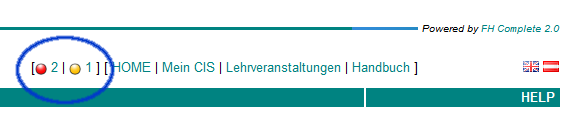
\includegraphics[width=0.70\textwidth]{CIS_Ampelsystem_Ampelicons.png}
	\caption{Offene Ampeln werden in der Titelleiste angezeigt}
	\label{ampel_icons}
\end{figure}

Nach dem Klicken auf eine offene Ampel wird eine �bersichtsseite geladen, auf der nun jede Meldung einzeln best�tigt werden kann (siehe Abbildung \ref{ampel_uebersicht}).
Eine Meldung kann dabei von folgenden Parametern eingeschr�nkt werden:

\begin{description}
	\item[Beschreibung:] Titel und Inhalt der Meldung.
	\item[Zielgruppe:] F�r eine Meldung kann genau definiert werden, wer diese angezeigt bekommen soll. Dies k�nnen definierte Personengruppen (MitarbeiterInnen, Studierende, ...) und/oder einzelne Personen sein.
	\item[Deadline:] Gibt an, ab wann das Datum einer Meldung als "`�berschritten"' gilt. Ab diesem Zeitpunkt, wird die Ampel auf "`rot"' gesetzt.
	\item[Vorlaufzeit (in Tagen):] Gibt an, ab wann die Meldung angezeigt und als "`gelb"' markiert wird.
	\item[Verfallzeit (in Tagen):] Gibt an, ab wann die Meldung nicht mehr angezeigt wird. Dabei spielt es keine Rolle, ob die Meldung best�tigt wurde oder nicht.
\end{description}

\begin{figure}
	\centering
	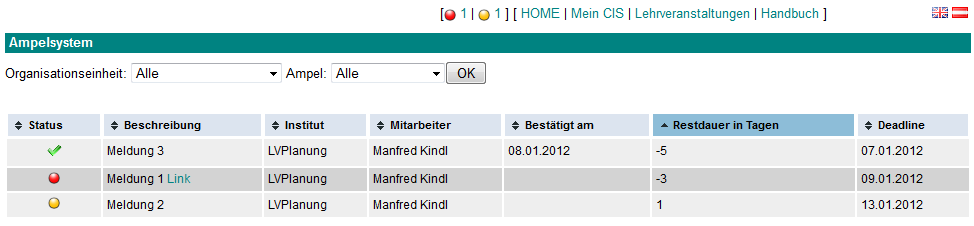
\includegraphics[width=1\textwidth]{CIS_Ampelsystem_Ampeluebersicht.png}
	\caption{�bersicht zum Best�tigen der Meldungen}
	\label{ampel_uebersicht}
\end{figure}

\section{Ampel�bersicht}
\label{ampeluebersicht}

Wie in Abbildung \ref{ampel_uebersicht} gezeigt, werden auf der �bersichtsseite alle Meldungen untereinander angef�hrt. Dabei werden Meldungen VOR der Deadline mit einer gelben Ampel gekennzeichnet, Meldungen, die die Deadline �berschritten haben, werden mit einer roten Ampel gekennzeichnet und best�tigte Meldungen werden mit einem gr�nen Haken markiert.
Wenn eine Meldung die Verfallszeit erreicht hat, wird diese nicht mehr angezeigt (Egal ob best�tigt oder nicht).

\subsection{Meldung best�tigen}

Klicken Sie in der letzten Spalte auf "`best�tigen"' um eine Meldung zu best�tigen. Daraufhin wird die Meldung mit einem gr�nen Haken markiert und bis zum Verfallsdatum als "`best�tigt"' angezeigt.

\section{Sonstiges}

Sie k�nnen die Liste durch Klicken auf die Spalten�berschriften sortieren.

\section{Ampel�bersicht f�r LeiterInnen}
\label{ampeluebersicht_leiterinnen}

Unter "`Mein CIS -> Ampel-�bersicht"' k�nnen Sie bei entsprechender Berechtigung den Status aller Meldungen einsehen.
Damit haben Sie einen �berblick, welche Personen eine entsprechende Meldung best�tigt haben oder nicht.
Sie k�nnen die Liste nach Organisationseinheit und/oder Bezeichnung der Ampel filtern und durch Klicken auf die Spalten�berschrift sortieren.

In der Spalte "`Best�tigt am"' ist ersichtlich, wann die Meldung best�tigt wurde.
Die Spalte "`Restdauer in Tagen"' gibt an, wann die Deadline der Meldung erreicht wird bzw. bei negativen Zahlen, um wieviele Tage die Deadline �berschritten wurde.
\chapter{News}
\section{Allgemeines}

Im CIS gibt es verschieden Ansichten f�r News (im Bereich der LV-News auch Pinboard genannt). Auf der Startseite befindet sich die Ansicht f�r "`allgemeine News"'. Des weiteren gibt es Ansichten f�r die einzelnen Organisationseinheiten (Studiengang, Institut, ...). Hier werden die allgemeinen mit den spezifischen News gemischt angezeigt.

Die Berechtigungen f�r das Eintragen von News h�ngen von den Berechtigungen des Benutzers ab.
LektorInnen d�rfen News zu Organisationseinheiten (z.B. Studieng�nge) unbegrenzt auf dem Pinboard einstellen.
Berechtigungen f�r allgemeine News werden von der Systemadministration einzeln an MitarbeiterInnen vergeben.

\section{Richtlinien zu Newseintr�gen}
\label{richtlinien_newseintraege}

Folgende Richtlinien sind f�r das Einstellen von Newseintr�gen zu beachten:
\minisec{Allgemeine News}
Allgemeine News sollten zum einen MitarbeiterInnen UND Studierende betreffen und zum Anderen in direktem Zusammenhang mit unserer Organisation stehen. Auf keinen Fall soll hier eine Werbeplattform f�r externe Veranstaltungen entstehen. 

\idee{Allgemeine News werden von der Infrastruktur �bersetzt}

\minisec{OE News}
News in den Organisationseinheiten richten sich an MitarbeiterInnen und Studierende innerhalb der OE.
OE-News werden nicht automatisch �bersetzt. Die OE hat aber die M�glichkeit dies selbst zu tun.
Siehe dazu Kapitel \ref{uebersetzung_eines_neweintrags}

\section{Erstellung}

\subsection{So erstellen Sie einen allgemeinen Newseintrag}
\label{allgemeinen_Newseintrag_erstellen}

Die Newsverwaltung f�r die allgemeinen News befindet sich im Punkt "`Infrastruktur"' unter "`Verwaltungstools"'.

\begin{figure}
	\centering
	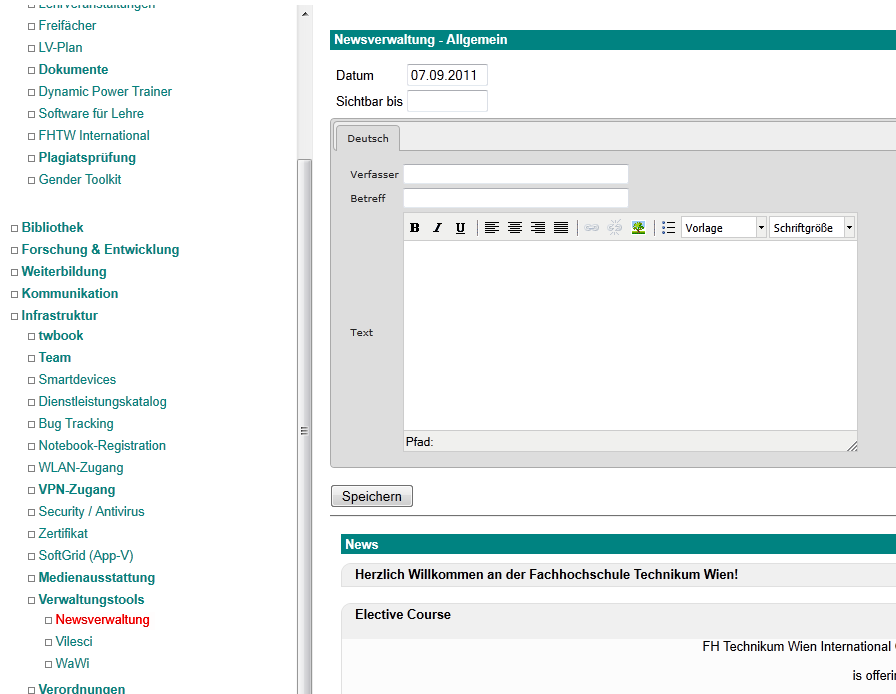
\includegraphics[width=0.70\textwidth]{CIS_Newsverwaltung_01.png}
	\caption{CIS allgemeine Newsverwaltung}
	\label{CIS_newsverwaltung}
\end{figure}

		\begin{itemize}
			\item Geben Sie neben "`Datum"' das Datum ein, ab wann der Eintrag sichtbar sein soll (Standardeinstellung: heute).
			\item Geben Sie optional ein Enddatum (max. 30 Tage) ein, bis wann der Eintrag aufscheinen soll (Ohne Eintrag 30 Tage).
			\item Tragen Sie eine/n VerfasserIn ein, der/die im Newseintrag in der Titelzeile aufscheinen soll.
			\item Geben Sie dem Eintrag einen aussagekr�ftigen Betreff.
			\item Geben Sie den gew�nschten Text ein und formatieren Sie ihn mit den entsprechenden Buttons. Die Funktion der Buttons wird erkl�rt, wenn Sie mit dem Mauszeiger dar�ber stehen.
			Sie k�nnen die Gr��e des Bearbeitungsfensters beliebig ver�ndern, indem Sie die schraffierte Fl�che rechts unten mit der Maus verschieben.
			\item Zuletzt speichern Sie den Eintrag durch dr�cken des Buttons "`Speichern"'
			\item Wie Sie eine �bersetzung des Eintrags vornehmen k�nnen, erfahren Sie in Kapitel \ref{uebersetzung_eines_neweintrags}.
		\end{itemize}
		
\subsection{So erstellen Sie einen OE-spezifischen Newseintrag}
Die Newsverwaltung f�r die OE-News finden Sie durch klicken auf den Men�punkt "`Lehrveranstaltungen"' und anschlie�ender Auswahl des gew�nschten Studiengangs.
Klicken Sie anschlie�end auf "`Lektorenbereich"' und "`Pinboard administration"'.

\begin{figure}
	\centering
	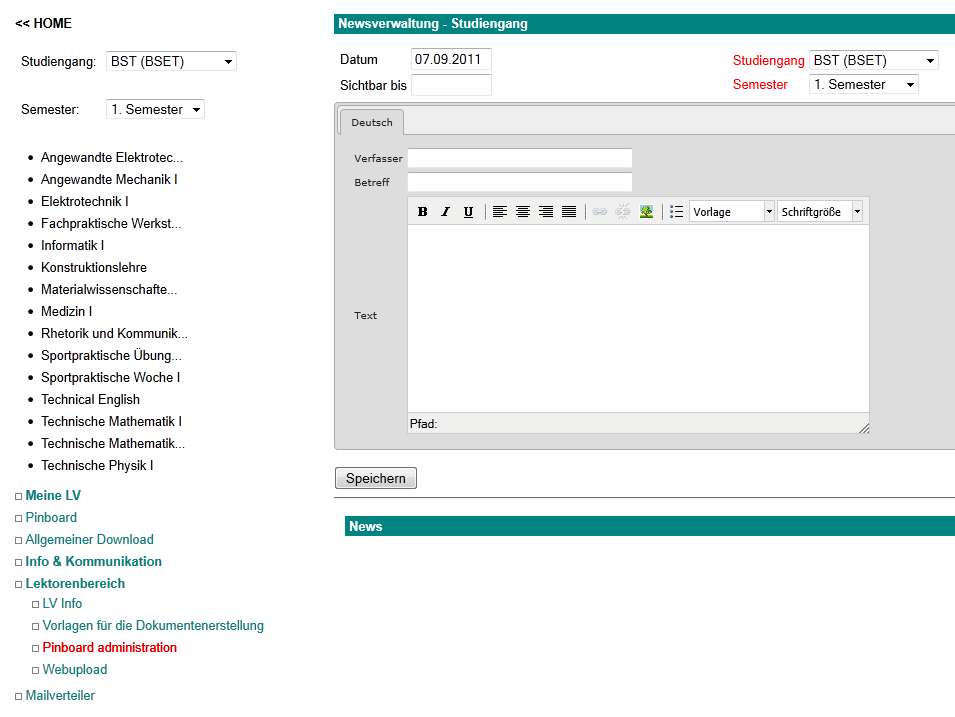
\includegraphics[width=0.70\textwidth]{CIS_Newsverwaltung_03.png}
	\caption{CIS Newsverwaltung f�r OE}
	\label{CIS_newsverwaltung}
\end{figure}

Verfahren Sie hier mit dem Newseintrag genauso wie in Kapitel \ref{allgemeinen_Newseintrag_erstellen} beschrieben mit dem einzigen Unterschied, dass Sie in der Kopfzeile noch zus�tzlich den betreffenden Studiengang bzw. das gew�nschte Semester ausw�hlen k�nnen, f�r das der Eintrag sichtbar sein soll.

\subsection{So legen Sie eine �bersetzung f�r einen Newseintrag an}
\label{uebersetzung_eines_neweintrags}
�bersetzungen f�r allgemeine News (Gilt nicht f�r OE-News) werden von der Infrastruktur automatisch an den �bersetzer weitergeleitet und danach eingegeben.
Falls Sie einen Beitrag dennoch gleich selbst �bersetzen m�chten oder diese f�r eine OE-News tun wollen, gehen Sie bitte wie folgt vor:
(Sehen Sie dazu auch Kapitel \ref{richtlinien_newseintraege} Richtlinien zu Newseintr�gen)
		\begin{itemize}
			\item Nachdem Sie einen deutschen Eintrag gespeichert haben, erschein nebem dem Registerblatt "`Deutsch"' ein +-Symbol.
				\begin{figure}
				\centering
				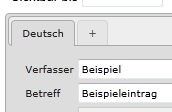
\includegraphics[width=0.30\textwidth]{CIS_Newsverwaltung_02.png}
				\end{figure}
			\item Klicken Sie auf "`+"' und w�hlen Sie die gew�nschte Sprache aus.
			\item Verfahren Sie wie in Kapitel \ref{allgemeinen_Newseintrag_erstellen} beschrieben mit dem Eintrag.
			\item Zuletzt speichern Sie den Eintrag durch Dr�cken den Buttons "`Speichern"'.
		\end{itemize}
Wird nun die CIS-Seite in einer anderen Sprache aufgerufen, erscheint der entsprechende Beitrag in der jeweiligen Sprache, falls eine solche �bersetzung vorhanden ist.
Gibt es zu einem deutschsprachigen Eintrag keine entsprechende �bersetzung, wird der deutsche Inhalt des Newseintrags angezeigt.


\chapter{Lehre}
\label{lehre}
\section{Allgemeines}

Der Bereich "`Lehre"' beinhaltet die wichtigsten Verkn�pfungen f�r den Studienalltag.
Hier k�nnen Informationen zu den Lehrveranstaltungen, der Stundenplan, Anwesenheitslisten und Semesterpl�ne abgerufen werden.

\section{Lehrveranstaltungen}
\label{lehre_lehrveranstaltungen}

Auf der Seite der Lehrveranstaltungen k�nnen Sie zun�chst den Studiengang und das Semester w�hlen, dessen Inhalt angezeigt werden soll.

\begin{figure}
	\centering
	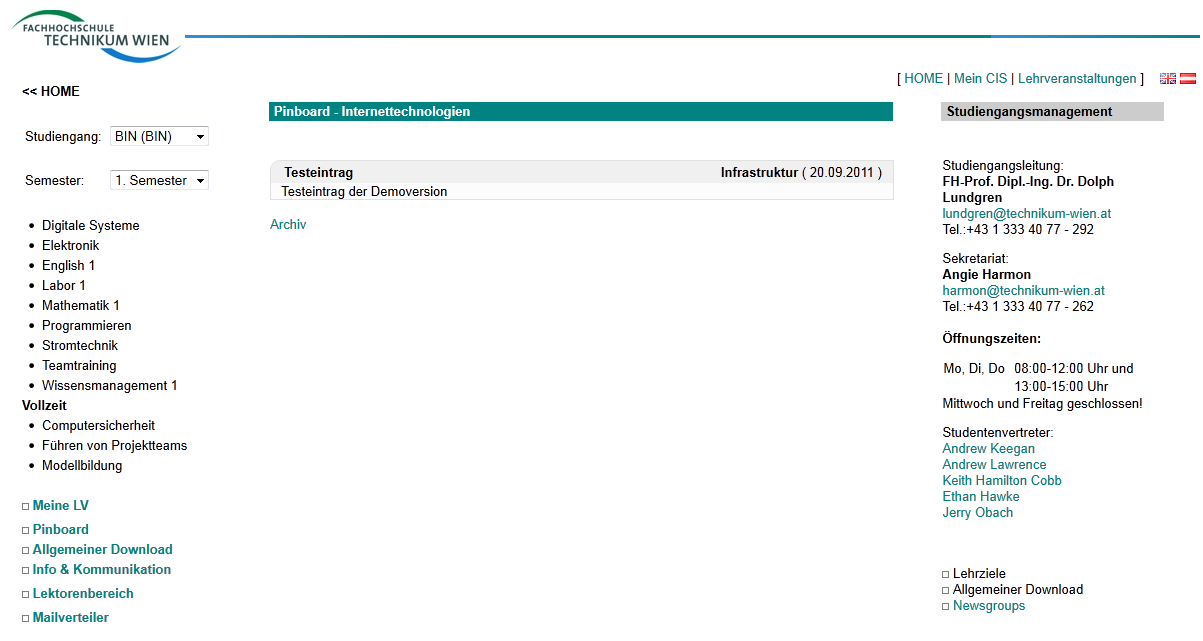
\includegraphics[width=0.70\textwidth]{CIS_Lehrveranstaltungen.png}
	\caption{CIS Lehrveranstaltungen}
	\label{CIS_lehrveranstaltungen}
\end{figure}

Die News im Hauptfenster setzen sich zusammen aus den allgemeinen News und spezifischen News entsprechend dem gew�hlten Studiengang. Sind keine spezifischen News vorhanden, sind nur allgemeine Newseintr�ge sichtbar.

Nach der Auswahl des gew�nschten Studiengangs, werden alle zugeh�rigen aktiven Lehrveranstaltungen aufgelistet.
Wenn Sie eine davon ausw�hlen, erscheint im Hauptfenster die �bersicht mit allen Tools und Informationen, die zu dieser LV zur Verf�gung stehen. (siehe Abbildung \ref{CIS_lehrveranstaltungen})

\begin{figure}
	\centering
	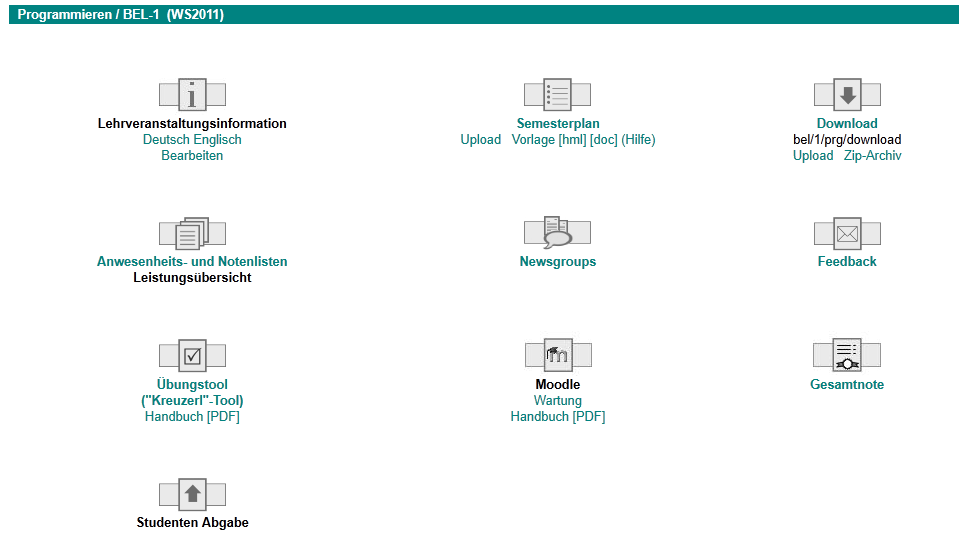
\includegraphics[width=0.70\textwidth]{CIS_Lehrveranstaltungen_Icons.png}
	\caption{CIS Lehrveranstaltungen Details}
	\label{CIS_lehrveranstaltungen}
\end{figure}

Hier k�nnen Sie LV-Infos, den Semesterplan oder den Downloadbereich einsehen und Anwesenheitslisten generieren lassen.
Zur Unterst�tzung der Lehre stehen Ihnen au�erdem 3 Werkzeuge zur Verf�gung: Das �bungstool, das Abgabe-Tool oder die eLearning-Plattform Moodle.

Im linken Men� finden Sie dar�ber hinaus die Bereiche:
\begin{description}
	\item [Meine LV:] Das sind jene Lehrveranstaltungen, die Sie pers�nlich als LektorIn bzw. Studierenden betreffen.
	\item [Pinboard:] Die Newsansicht mit aktuellen Informationen.
	\item [Allgemeiner Download:] Ein Link zum Downloadbereich des Studiengangs.
	\item [Info \& Kommunikation:] Hier ist ein Link zum Stundenplan sowie zum Webmail zur Verwaltung Ihrer E-Mails.
	\item [Lektorenbereich:] Mit der entsprechenden Berechtigung k�nnen Sie hier die LV-Infos bearbeiten, Unterlagen hochladen und Newseintr�ge erstellen.
	\item [Mailverteiler:] Hier finden Sie eine �bersicht aller Mailverteiler an der FHTW. Gro�e Verteiler sind standardm��ig f�r Studierende gesperrt.
\end{description}

\section{Freif�cher}
\label{lehre_freifaecher}

Studierende k�nnen aus allen angebotenen Freif�chern beliebig w�hlen. Die Terminvereinbarung obligt dem/der LektorIn.
Die Seite der Freif�cher unterscheidet sich nur unwesentlich von der der Lehrveranstaltungen.
Auch hier k�nnen LV-Infos eingetragen, Semesterpl�ne und Anwesenheitslisten gedruckt werden.

Links finden Sie den Punkt "`Anmeldung"' wo Sie alle gew�nschten Freif�cher markieren und sich mit dem Button "`Speichern"' anmelden k�nnen.
In der "`�bersicht"' k�nnen Sie Einblick in die derzeitigen Anmeldungen nehmen.

Eine Abmeldung f�r ein Freifach ist derzeit nur �ber die Studiengangsassistenz m�glich.

\section{LV-Plan}
\label{lehre_lvplan}

Der LV-Plan ist der Stundenplan der FHTW.
Sie k�nnen zwischen Ihrem pers�nlichen Plan, dem Saalplan, dem Lektorenplan oder dem Lehrverbandsplan w�hlen.

\begin{figure}
	\centering
	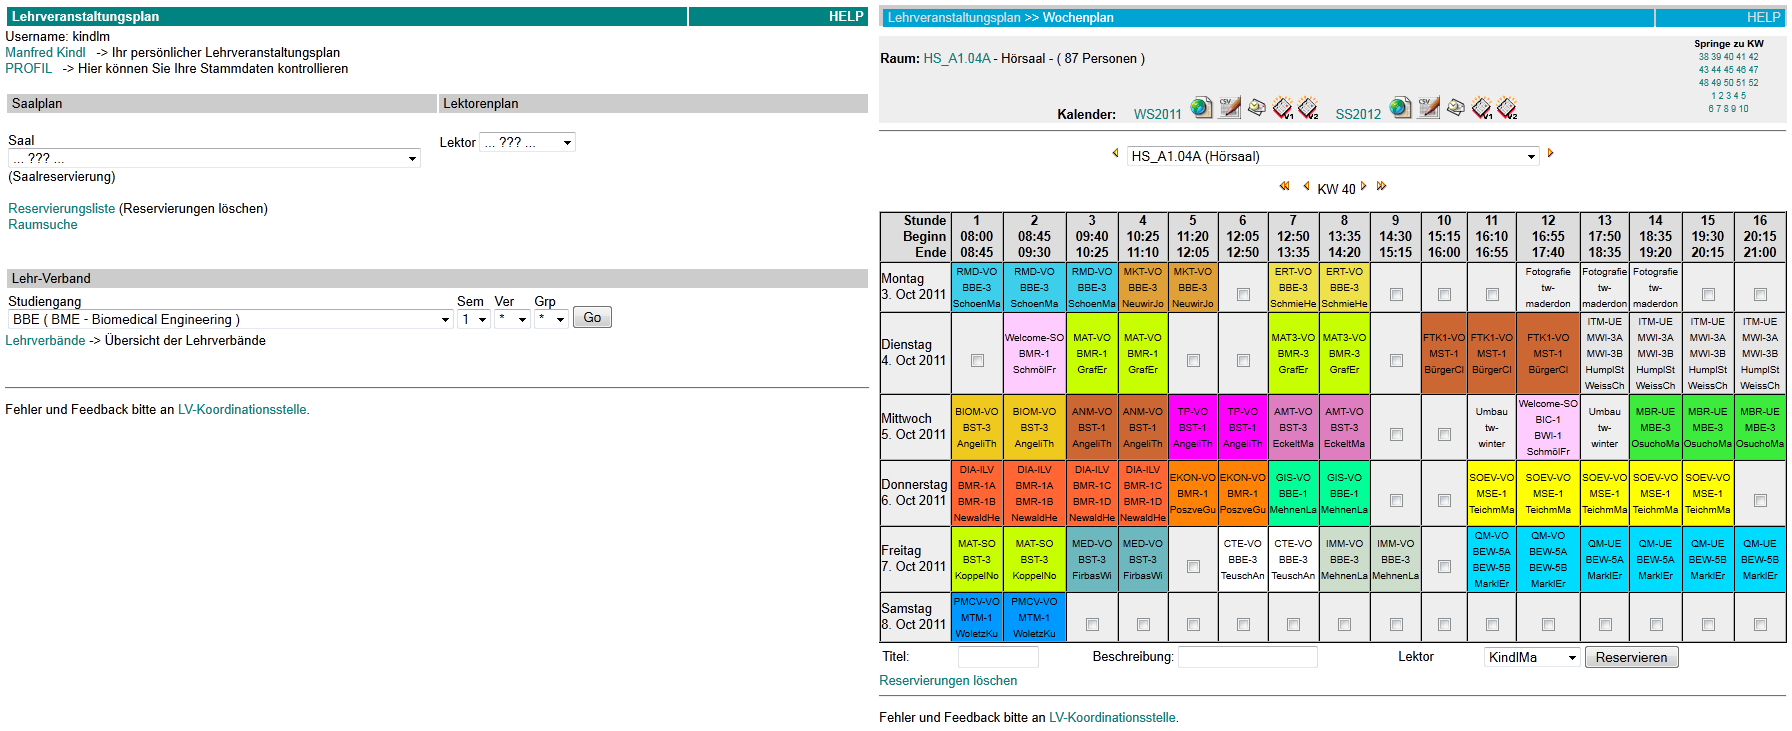
\includegraphics[width=1\textwidth]{CIS_Lvplan.png}
	\caption{CIS Lehrveranstaltungsplan}
	\label{CIS_lvplan}
\end{figure}

\begin{description}
	\item [Pers�nlicher Lehrveranstaltungsplan:] Hier sehen Sie jene LV's die Sie pers�nlich betreffen. Sie sehen nur die Stunden Ihrer zugeteilten Gruppe, eventuell gew�hlte Freif�cher und Ihre eigenen  Reservierungen.
	\item [Saalplan:] In der Liste finden Sie alle Unterrichtsr�ume an der FHTW und k�nnen sich dann die jeweilige Saalbelegung ansehen. �ber den Saalplan k�nnen Sie - bei entsprechender Berechtigung - auch Reservierungen vornehmen.
	\item [Lektorenplan:] Zeigt Ihnen den Stundenplan eines/einer Lektors/Lektorin.
	\item [Lehr-Verband:] Hier k�nnen Sie die Pl�ne jedes Studiengangs optional auf Semester, Verband und Gruppe eingeschr�nkt einsehen.
\end{description}

\subsection{Die Kalenderansicht}

Hier k�nnen Sie durch klicken auf die Pfeile eine bzw. vier Wochen vor- bzw. zur�ckbl�ttern.
In der Saalplan-Ansicht haben Sie noch zus�tzlich ein Dropdown um zwischen den R�umen bl�ttern zu k�nnen.
Wenn Sie eine eingetragene Einheit anklicken �ffnet sich ein Detailfenster, dem Sie zus�tzliche Informationen entnehmen k�nnen.

Au�erdem haben Sie die M�glichkeit, sich den Semesterplan (�bersicht mit allen Wochen untereinander) durch klicken auf WS20xx bzw SS20xx zu laden.

Mit den 5 Icons neben dem jeweiligen Semesterplan, k�nnen Sie sich den LV-Plan in andere Clients (zB Outlook, Sunbird, Smartphone, ...) exportieren.

\subsection{Reservierung vornehmen}

Um einen Raum reservieren zu k�nnen, ben�tigen Sie die entsprechenden Rechte (Mitarbeiter, Lektoren, Studentenvertreter).
W�hlen Sie aus dem Saalplan den gew�nschten Ort und markieren Sie mit den Checkboxen jene Einheiten, die Sie reservieren m�chten.
Geben Sie danach einen Titel und einen kurzen Beschreibungstext ein, wof�r Sie die Einheit reservieren m�chten.
Klicken Sie abschlie�end auf den Button "`Reservieren"'.

\info{Die reservierte Einheit ist nur im Raumplan und in Ihrem pers�nlichen Plan sichtbar. Wenn Sie die Reservierung f�r einen Studiengang, Semester oder Verband sichbar machen wollen, kontaktieren Sie bitte die Lehrveranstaltungsplanung}

\subsection{Reservierung l�schen}

Sie k�nnen sich Ihre Reservierungen durch klicken auf "`Reservierungsliste"' im Hauptmen� bzw. "`Reservierungen l�schen"' im Saalplan ansehen und dort ggf. l�schen.

\subsection{Rauminformationen}

Wenn Sie sich im Saalplan befinden, k�nnen Sie links oben die Bezeichnung des Raumes anklicken.
Sie werden danach auf eine Seite weitergeleitet, auf der Sie detaillierte Informationen zur Raumausstattung, Bilder und Lageinformationen finden.

\section{Dokumente}

Hier finden Sie wichtige und hilfreiche Dokumente rund um den Studienalltag. Je nach Berechtigung k�nnen Sie auf unterschiedliche Ordner zugreifen und Dateien herunterladen.

\section{Software f�r die Lehre}

Hier finden Sie Software, die Sie zur Unterst�tzung der Lehre einsetzen k�nnen.

\begin{description}
	\item [Softgrid:] Ist eine umgebungsunabh�ngige Virtualisierungssoftware mit der Apllikationen nicht mehr auf dem Endger�t installiert, sondern jederzeit zentral zur Verf�gung gestellt werden. Das lokale Zwischenspeichern (Cachen) der ben�tigten Anwendungen versetzt Sie in die Lage, diese Anwendungen "`mitzunehmen"' und bis zu 40 Tage offline zu benutzen. Details zur Installation finden Sie im Bereich "`Infrastruktur"'.
	\item [Dynamic Power Trainer:] Ist eine professionelle Authoring Software, mit der Sie eLearning Kurse erstellen k�nnen.
	\item [Moodle:] Ist ein objektorientiertes Kursmanagementsystem, eine Lernplattform auf Open-Source-Basis. Die Software bietet die M�glichkeiten zur Unterst�tzung kooperativer Lehr- und Lernmethoden.
\end{description}

\section{Plagiatspr�fung}

Hier k�nnen sowohl Studierende als auch LektorInnen ihre wissenschaftlichen Arbeiten zur Plagiatspr�fung durch die externe Plattform "`Ephorus"' abgeben.
\chapter{Urlaubsverwaltung}
\label{urlaubsverwaltung}
\section{Allgemeines}

Die Urlaubsverwaltung ist unter "`Mein CIS"' Urlaubstool zu finden.
Das Urlaubstool dient als Erweiterung der Zeitsperren (siehe Kapitel \ref{zeitsperren_zeitwuensche}), um diese leichter und �bersichtlicher eintragen zu k�nnen.

\begin{itemize}
	\item Der Abrechnungszeitraum f�r die Urlaubserfassung ist von 01.09. eines Jahres bis zum 31.08. des Folgejahres.
	\item Der Urlaubsanspruch eines/einer MitarbeiterIn wird von der Gesch�ftsstelle administriert und gewartet.
	\item Der/die MitarbeiterIn tr�gt im Laufe des Jahres im Urlaubstool seine/ihre gew�nschten Urlaubstage ein.
	\item Der/die - in der Datenbank zugeteilte - InstitutsleiterIn bzw. Vorgesetzte erh�lt daraufhin eine E-Mail mit einem Freigabeansuchen. Nach der Freigabe kann der eingetragene Urlaub nicht mehr durch den/die MitarbeiterIn bearbeitet werden.
	\item Mit Stichtag 31.08. wird der aktuelle Urlaubsanspruch ermittelt. Dazu tr�gt der/die InstitutsleiterIn/Vorgesetzte die aktuellen Resturlaubstage in das System ein. Diese werden mit dem derzeitigen Urlaubsanspruch addiert und ergeben, abz�glich des aktuell gebuchten Urlaubs, den Urlaubsanspruch ab 01.09.
	\item Der/die MitarbeiterIn kann diese Berechnung auf der CIS-Seite einsehen.
	\item Bei fehlender oder falscher Institutszuordnung wenden Sie sich bitte an die Personalabteilung. 
\end{itemize}

\begin{figure}
	\centering
	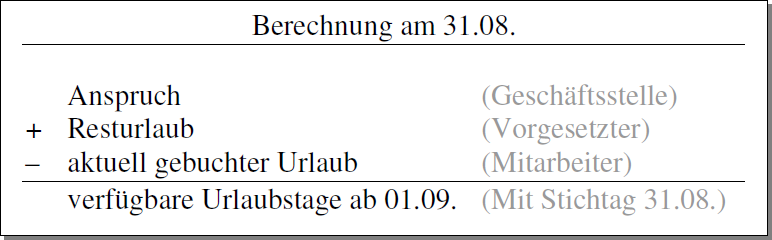
\includegraphics[width=0.70\textwidth]{CIS_Urlaubstool_Berechnung.png}
	\caption{Berechnung der Urlaubstage}
\end{figure}

\section{Verwendung des Tools}

Das Urlaubstool wird �ber die CIS-Seite aufgerufen und dient als Erweiterung der bisherigen Eingabemaske der Zeitsperren. Sie k�nnen weiterhin Zeitsperren wie gewohnt eintragen und bearbeiten.
Wir empfehlen, Mozilla Firefox oder SeaMonkey als Browser zu verwenden.

\subsection{Buchen eines Urlaubs}

Der �bersicht oben links (siehe Abbildung \ref{CIS_urlaubstool_eintragungen}) k�nnen Sie Ihren aktuellen Urlaubsanspruch und dessen Berechnung entnehmen. Mit dem Hilfe-Button erhalten Sie eine detaillierte
Erl�uterung der Berechnung.

\begin{figure}
	\centering
	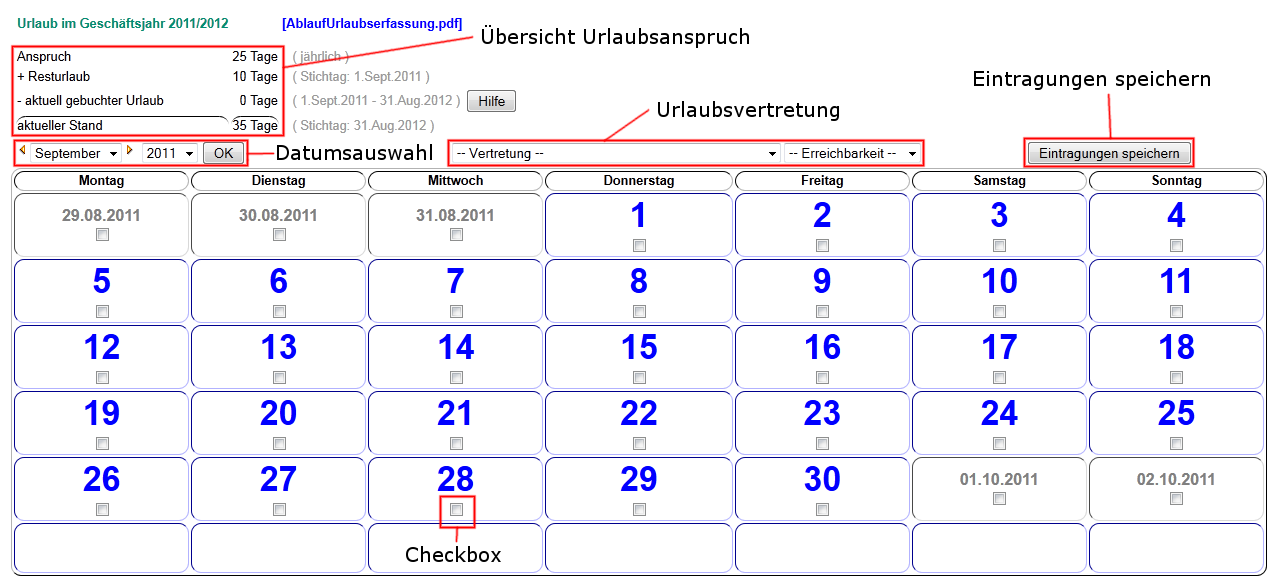
\includegraphics[width=1\textwidth]{CIS_Urlaubstool_Eintragungen.png}
	\caption{Eintragungen speichern}
	\label{CIS_urlaubstool_eintragungen}
\end{figure}

W�hlen Sie nun das gew�nschte Monat und Jahr aus, in dem Sie den Urlaub eintragen m�chten. Dies k�nnen Sie direkt mittels Auswahl aus den Drop-Down-Feldern und \textbf{dr�cken des OK-Buttons} oder durch Bl�ttern mit den gelben Pfeiltasten.

Sie sehen unter jedem Wochentag Checkboxen, die Sie durch einen einfachen Klick mit der Maustaste an- und abw�hlen k�nnen. Markieren Sie nun auf diese Weise die Tage, an denen Sie Ihren Urlaub konsumieren m�chten.

\achtung{Es werden zur Zeit noch keine Feiertage angezeigt. Kontrollieren Sie bitte selbstst�ndig, ob ein Feiertag innerhalb Ihres Urlaubs liegt.}

W�hlen Sie nun aus den Drop-Down-Feldern Ihre Urlaubsvertretung aus und wie Sie f�r die Zeit Ihres Urlaubs erreichbar sind. 
Wenn Sie nichts angeben, wird automatisch "`Nicht erreichbar!"' gespeichert. Dr�cken Sie nun \textbf{Eintragungen speichern}. 

Der gebuchte Urlaub erscheint nun in Hellgr�n im Kalender. Gleichzeitig wird eine
E-Mail mit dem Freigabeansuchen an Ihren Vorgesetzten versendet, was Ihnen auch unterhalb des Kalenders durch einen roten Infotext best�tigt wird.

\info{Sollte kein/e Vorgesetzte/r in der Datenbank zugeordnet sein, so steht dies ebenfalls im Infotext. Kontaktieren Sie in diesem Fall bitte die Personalabteilung.}

Wenn Sie mit dem Cursor auf einem gebuchten Urlaub zu stehen kommen (auf der Zahl) erscheint im Quickinfo die gespeicherte Vertretung und Erreichbarkeit.

\begin{figure}
	\centering
	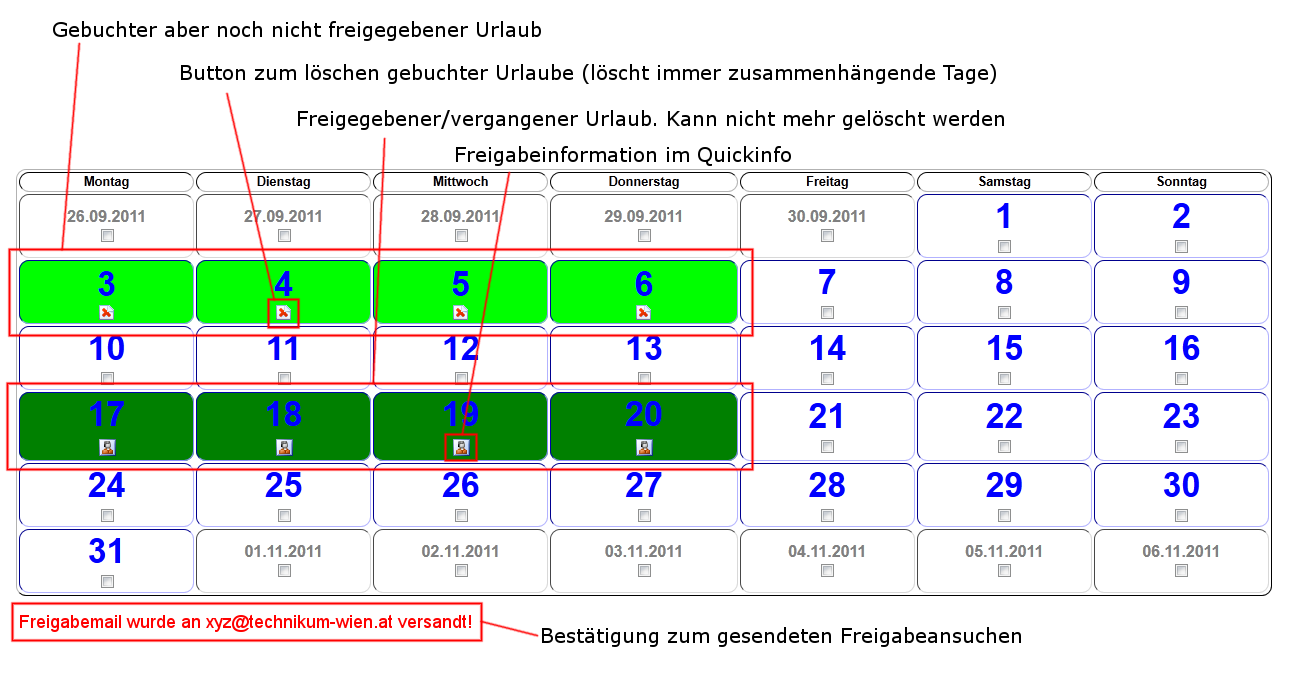
\includegraphics[width=1\textwidth]{CIS_Urlaubstool_Buchungen.png}
	\caption{Eingetragener Urlaub}
	\label{CIS_urlaubstool_buchungen}
\end{figure}

\section{L�schen eines gebuchten Urlaubs}

Einen gebuchten und noch NICHT freigegebenen Urlaub, k�nnen Sie durch klicken auf das x unterhalb eines jeden Eintrags l�schen.
Zusammenh�ngende (aufeinander folgende) Tage werden als solche gespeichert und auch entsprechend wieder gel�scht. Ein Klick auf den L�schen-Button in Abbildung \ref{CIS_urlaubstool_buchungen},
w�rde also den Urlaub vom 03.-06.August l�schen.

\textit{Bitte buchen Sie Ihren Urlaub �berlegt, um Ihrem/Ihrer Vorgesetzten eine Flut an Mails zu ersparen und unn�tige Verwirrungen zu vermeiden.}

\section{Freigegebener Urlaub}

Nachdem Ihr/e Vorgesetzte/r Ihren gew�nschten Urlaub freigegeben hat, erscheint er im Urlaubstool dunkelgr�n und kann nicht mehr von Ihnen gel�scht werden.
Das L�schen-Symbol ist nun durch ein Informations-Icon ersetzt worden und im Quickinfo des Symbols erhalten Sie die Information, wann und von wem der Urlaub freigegeben worden ist.

\achtung{Wenn Sie nachtr�glich einen Urlaub in der Vergangenheit buchen (vor dem heutigen Datum), wird dieser automatisch als freigegeben markiert und kann nicht mehr gel�scht werden.}


\chapter{Zeitsperren/Zeitw�nsche}
\label{zeitsperren_zeitwuensche}

\section{Allgemeines}

Die Zeitw�nsche bzw. Zeitsperren finden Sie unter dem Punkt "`Mein CIS"'.
Sie dienen prim�r zur Unterst�zung der LV-Planung um dort Verf�gbarkeiten bzw. Terminvorlieben anzuzeigen.
Die eingetragenen Urlaube im Urlaubstool (siehe Kapitel \ref{urlaubsverwaltung}) werden ebenfalls als Zeitsperre im System hinterlegt und k�nnen dort als solche bearbeitet werden.

\section{Zeitsperren}
\label{zeitsperren}

Die Zeitsperren sind - anders als die Zeitw�nsche - zum punktuellen Sperren bestimmter Termine gedacht.
Eine Zeitsperre wird durch ein genaues Datum (von-bis) und eine Uhrzeit (von-bis) begrenzt und kann dar�ber hinaus mit optionalen Zusatzangaben (zB. Grund, Vertretung,...) versehen werden.

Zeitsperren sind zB. daf�r gedacht, Zeitausgleiche, Konferenzen, Krankenst�nde, Dienstreisen und dgl. einzutragen (siehe Abbildung \ref{eingabemaske_zeitsperren}).

\begin{itemize}
	\item W�hlen Sie dazu einen "`Grund"' aus dem DropDown-Feld und geben Sie der Zeitsperre eine aussagekr�ftige Bezeichnung.
	\item Bei "`Von"' und "`Bis"' tragen Sie bitte das Datum und optional auch die Einheiten ein, welche Sie verhindert sind.
	\item Neben "`Erreichbarkeit"' k�nnen Sie ausw�hlen, ob Sie w�hrend Ihrer Abwesenheit telefonisch, per Mail oder nicht erreichbar sind.
	\item Schlie�lich k�nnen Sie noch eine Person als Vertretung angeben.
	\item Mit "`Hinzuf�gen"' best�tigen und speichern Sie Ihre Eingaben.	
\end{itemize}

Wenn Sie als Grund der Zeitsperre "`Urlaub"' ausw�hlen, sind die Eintragungen gleichbedeutend mit jenen des Urlaubstools (siehe Kapitel \ref{urlaubsverwaltung}).
Die Zeitsperre durchl�uft deshalb ebenfalls den Weg �ber die Freigabe (mit Mailversand an den/die VorgesetzteN) und die Urlaubstage werden entsprechend den Eintragungen abgezogen.

\achtung{Es werden alle eingegebenen Tage bei der Urlaubsberechnung ber�cksichtigt. Daher m�ssen mehrt�gige Zeitsperren an Unterbrechungen wie Wochenenden oder Feiertagen unterteilt werden}


\begin{figure}
	\centering
	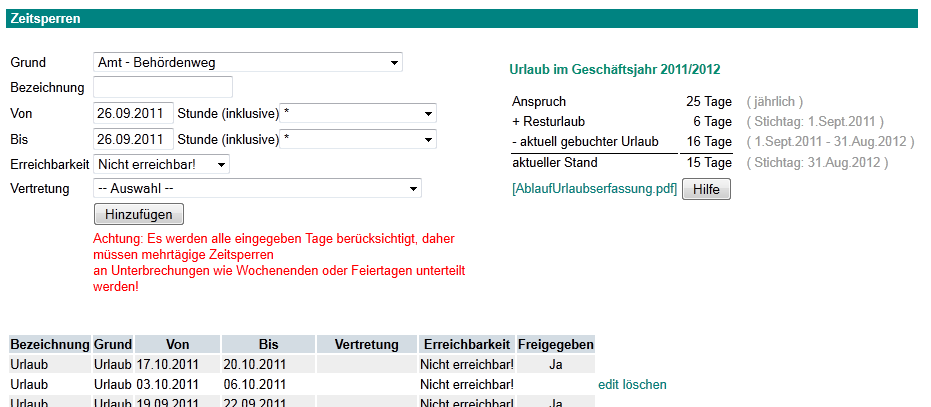
\includegraphics[width=0.70\textwidth]{CIS_Zeitsperre.png}
	\caption{Eingabemaske der Zeitsperren}
	\label{eingabemaske_zeitsperren}
\end{figure}

\subsection{Zeitsperren bearbeiten/l�schen}

Ihre eingegebenen Zeitsperren erscheinen in einer Liste unterhalb des Formulars.
Neben jeder Eintragung (ausgenommen freigegebene Urlaube) sehen Sie einen "`Edit"' und einen "`L�schen"' Button, mit dem Sie den jeweiligen Eintrag bearbeiten bzw. l�schen k�nnen.

Freigegebene Urlaube k�nnen von Ihnen weder bearbeitet noch gel�scht werden. Wenden Sie sich in diesem Fall an Ihre/Ihren VorgesetzteN.

\section{Zeitwunsch}

Der Zeitwunsch wird einmalig in ein statisches Normwochenraster eingetragen und soll eine grobe Schablone f�r die zeitlichen Verf�gbarkeiten der LektorInnen innerhalb einer "`normalen"' Woche sein.

Der/Die LektorIn kann f�r jeden Tag und jede Unterrichtseinheit einer Woche Gewichtungen von -2 bis +2 vergeben um so seine/ihre Verf�gbarkeit anzugeben.
Anhand des Zeitwunsches kann sich die LV-Planung orientieren, welche Terminvorlieben ein/eine LektorIn in einer Woche hat.

Der Zeitwunsch soll und kann NICHT genaue Verf�gbarkeiten abbilden, sondern bietet lediglich eine Orientierung.
Um detailliertere Terminvorgaben abzubilden, verwenden Sie bitte die Zeitsperren (Kapitel \ref{zeitsperren}).

\begin{figure}
	\centering
	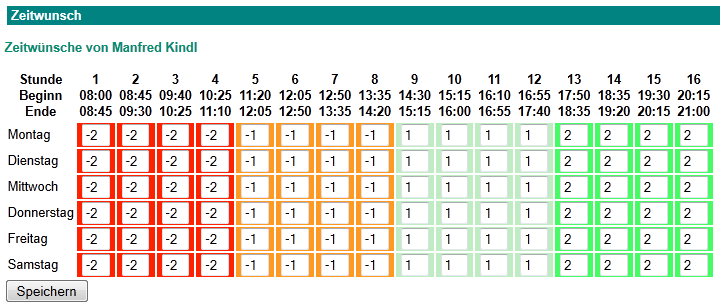
\includegraphics[width=0.70\textwidth]{CIS_Zeitwunsch.png}
	\caption{Zeitwunsch Eingabeformular}
\end{figure}

Standardeinstellung f�r den Zeitwunsch ist der Wert "`+1"' bei allen Einheiten.

Tragen Sie nun in jede Einheit, die Sie ver�ndern m�chten den gew�nschten Wert (-2 bis +2) ein und best�tigen Sie mit "`Speichern"'

\begin{tabular}{rll}
+2&...&hier m�chte ich unterrichten\\
+1&...&hier kann ich unterrichten\\
-1&...&hier unterrichte ich nur ungern\\
-2&...&hier kann ich gar nicht unterrichten\\
\end{tabular}

\idee{Sie k�nnen durch dr�cken der Tabulator-Taste auf Ihrer Tastatur rasch zwischen den Zellen wechseln}

Die Werte werden durch ein Farbsystem (von Rot bis Gr�n) im Hintergrund angezeigt.
 
Beachten Sie bitte folgendes:

\begin{enumerate}
	\item Verwenden Sie den Wert -2 nur, wenn Sie zu dieser Stunde wirklich nicht k�nnen, um eine bessere Optimierung zu erm�glichen.
	\item Die Zeitw�nsche sollen nach dem Fairplay-Prinzip gew�hlt werden, so dass mindestens dreimal so viele positiv bewertete Einheiten vorhanden sind, wie laut Lehrauftrag zu unterrichten w�ren. \\ Beispiel: Sie unterrichten 4 Stunden/Woche, dann sollten Sie mindestens 12 Stunden im Raster mit positiven Werten ausf�llen.
\end{enumerate} 

\chapter{Abgabetool f�r LektorInnen}
\label{Kapitel Aufruf}
Der Aufruf der LektorInnenoberfl�che erfolgt �ber cis.technikum-wien.at/Mein CIS/Bachelor- und Diplomarbeitsabgabe.

\section{�bersichtsliste der Betreuungen}
In der �bersichtsliste (siehe Abbildung \ref{abgabetool_uebersichtsliste}) finden sich alle Betreuungen von Bachelor- und Diplomarbeiten (im FAS unter Projektarbeit als �berbegriff zusammengefasst, daher der Name Projektarbeitsabgabe), deren Autorin oder Autor noch aktiv sind.

\begin {figure}
	\centering
	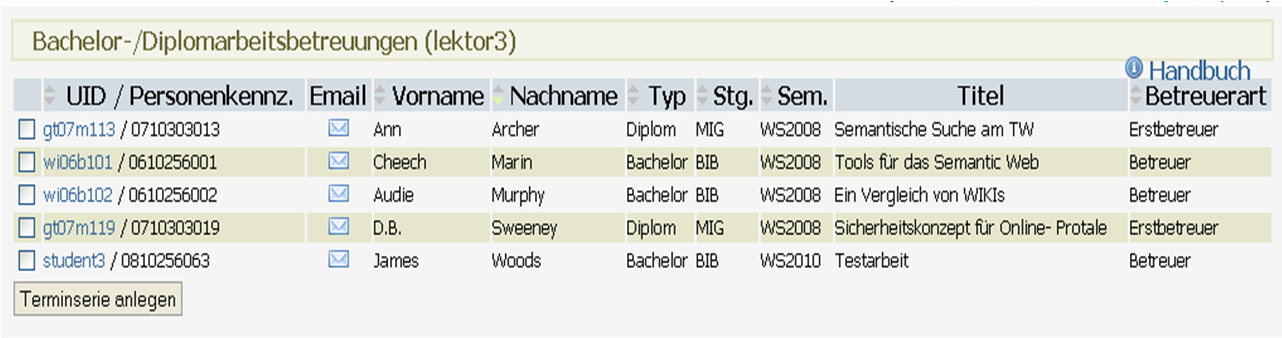
\includegraphics[width=1.0\textwidth]{abgabetool_uebersichtsliste}
	\caption{�bersichtsliste der betreuten Arbeiten}
	\label{abgabetool_uebersichtsliste}
\end {figure}

\subsection{Aufrufen der Termin�bersicht}
Durch Anklicken der UID der Studentin/des Studenten in der zweiten Spalte der �bersichtsliste werden die Termindetails im unteren Teil der Seite angezeigt (Siehe Abbildung \ref{abgabetool_terminverwaltung}).

\subsection{E-Mail an die Studentin/den Studenten}
Durch Anklicken des Briefsymbols in der dritten Spalte wird der E-Mailclient ge�ffnet und die Empf�nger- und Absenderadresse sowie \textit{Bachelorarbeitsbetreuung} bzw. \textit{Diplomarbeitsbetreuung} als Betreff werden vorausgef�llt.

\subsection{Termin f�r mehrere Studentinnen und Studenten ansetzen}
Es gibt auch die M�glichkeit, f�r mehrere Studentinnen und Studenten einen Termin zu setzen. Dazu m�ssen zuerst die betreffenden Zeilen durch Anklicken der Checkbox in der ersten Spalte markiert werden. Danach �ffnet ein Klick auf den Button \textit{Terminserie anlegen} eine Eingabemaske im unteren Teil des Browserfensters. Hier wird dann der Termin eingegeben und durch Dr�cken der Taste \textit{speichern} der Termin f�r alle zuvor markierten Betreuungen gespeichert.

\subsection{Aufruf der Anleitung}
Rechts neben der �berschrift \textit{Bachelor- /Diplomarbeitsbetreuungen} befindet sich ein blauer Icon mit einem weissen i. Durch einfaches Klicken darauf kann diese Anleitung als pdf-Datei aufgerufen werden.

\section{Termin�bersicht}

\begin {figure}
	\centering
	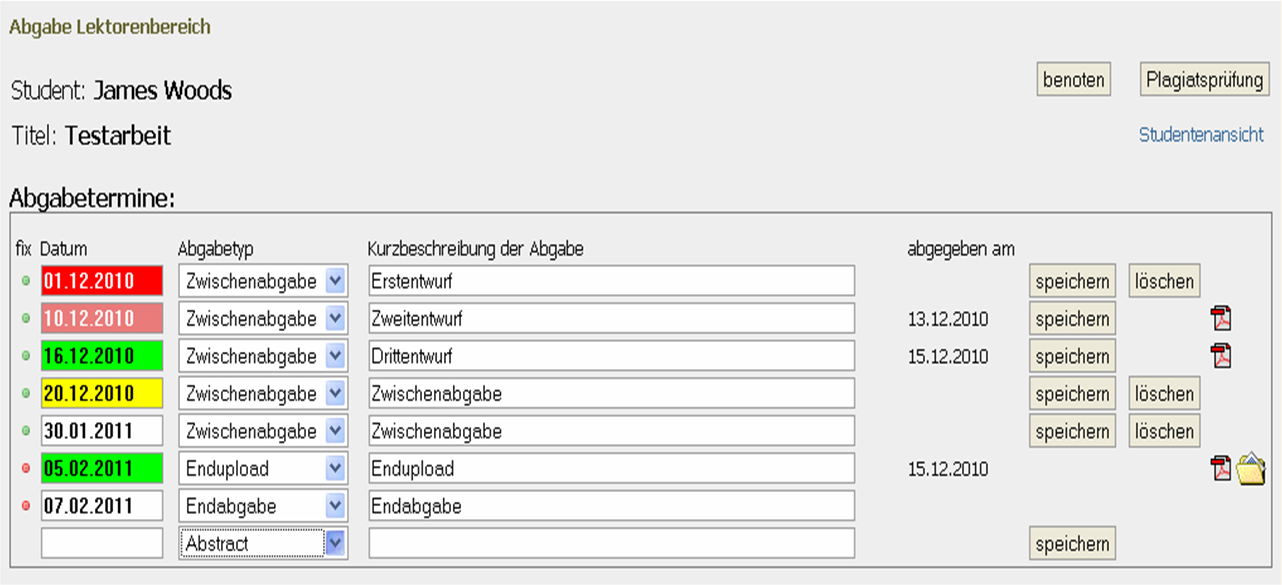
\includegraphics[width=1.0\textwidth]{abgabetool_terminverwaltung}
	\caption{Verwaltung und �bersicht der Termine}
	\label{abgabetool_terminverwaltung}
\end {figure}

\subsection{Termineingabe und -bearbeitung}

\begin{itemize}
	\item Termineingabe: Die unterste Zeile der Liste ist bis auf das Auswahlfeld \textit{Abgabetyp} leer und f�r die Eingabe eines neuen Termins vorgesehen. Geben Sie ein Datum ein, w�hlen Sie den Abgabetyp aus und geben Sie eine kurze Beschreibung der Abgabe ein. Abschlie�end wird mit einem Klick auf den Button \textit{speichern} der Termin eingetragen.
	\item Termin�nderung: Termineintr�ge k�nnen ge�ndert werden, indem Sie die Daten der betreffenden Zeile �ndern und anschlie�end \textit{speichern} dr�cken.
	\item Termin l�schen: Termin k�nnen durch Klicken auf die Taste \textit{l�schen} gel�scht werden. Ist bereits eine Abgabe erfolgt, kann ein Termin nicht mehr gel�scht werden.
	
	\info{�ber alle drei Aktionen wird die Studentin/der Student per Mail informiert}
	\item Die Assistenz kann fixe Termine vergeben, erkennbar an dem roten Bullet unter \textit{fix}. Liegt ein Termin in der Vergangenheit, kann die Studentin/der Student zu diesem nichts mehr hochladen. Soll dennoch etwas hochgeladen werden, mu� die Studentin/der Student bei der Studiengangsassistenz um eine Korrektur des Termins ansuchen.
	
	\info{Es k�nnen nur selbst angelegte Termine ge�ndert und gel�scht werden}
\end{itemize}

\subsection{Farbcode}

\begin{itemize}
	\item wei�:	"normaler" Termin
	\item gelb:	Termin innerhalb der n�chsten 12 Tage
	\item rot:	Termin �berschritten
	\item gr�n:	Abgabe erfolgt
	\item hellrot: Abgabe nach Termin 
\end{itemize}

\subsection{Download der Abgabe und Ansicht der Zusatzdaten}
Durch Klicken auf das Symbol 
\includegraphics{icon_pdf} wird ein Dialogfenster zum Speichern oder Betrachten der Abgabe dieses Termins ge�ffnet.
Bei der Endabgabe m�ssen von der Studentin/dem Studenten zus�tzlich Daten f�r die Publikationsdatenbank eingegeben werden. Diese sollten mittels dem Symbol 
\includegraphics{icon_ordner_endabgabe} vor der Benotung �berpr�ft werden.

\subsection{Benotung}
Rechts oben auf der Temin�bersicht befindet sich der Button \textit{benoten}, mit dem das Formular zur Benotung der Bachelor- bzw. Diplomarbeit aufgerufen werden kann. Die bereits verf�gbaren Daten wie die Daten der Studentin/des Studenten, Titel der Arbeit, Name der Begutachterin/des Begutachters sind bereits vorausgef�llt. Eingetragen m�ssen die verbalen Beschreibungen der Teilbenotungen und die Punkte der Teilbereiche. Aus den Punkten werden nach dem am Formular aufgef�hrten Schl�ssel die Noten sofort mit der Eingabe berechnet. 

Das Formular wird abschlie�end ausgedruckt und unterschrieben bei der Studiengangsassistenz abgegeben.

\subsection{Link zur Plagiatspr�fung}
Neben dem Button f�r das Benotungsformular befindet sich der Aufruf der Internetseite zur Plagiatspr�fung. Dort kann die abgegebene Arbeit hochgeladen werden.

\subsection{Studentenansicht}
Unterhalb des Links zur Plagiatspr�fung wird ein Link f�r die Studentenansicht angezeigt.
Hier wird die Abgabe aus Studentensicht angezeigt. Sie k�nnen von hier aus auch Arbeiten f�r die Studenten hochladen.

\subsection{Termin�bersicht f�r alle Termine}
Unterhalb der Liste der Studierenden gibt es die M�glichkeit, eine Liste mit allen Abgabeterminen der betreuten Studierenden zu erstellen. In dieser Liste werden alle Termine angezeigt die noch in der Zukunft liegen.

\subsection{Alte Arbeiten anzeigen}
Sie k�nnen sich die Termine und Arbeiten der abgeschlossenen Betreuungen einblenden, indem Sie unterhalb der Liste der Studierenden auf den Link "alle betreuten Arbeiten anzeigen" klicken. Es werden dann in der Liste, zus�tzlich zu den normalen Betreuungen, auch die Betreuungen angezeigt die bereits benotet wurden.
\chapter{Abgabetool f�r Studierende}
\label{Kapitel Aufruf}
Der Aufruf der Studierendenoberfl�che erfolgt �ber cis.technikum-wien.at/Mein CIS/Bachelor- und Diplomarbeitsabgabe.

\section{�bersichtsliste der Betreuungen}
In der �bersichtsliste (siehe Abbildung \ref{abgabetool_uebersicht_student}) finden sich alle Betreuungen von Bachelor- und Diplomarbeiten.

\begin {figure}
	\centering
	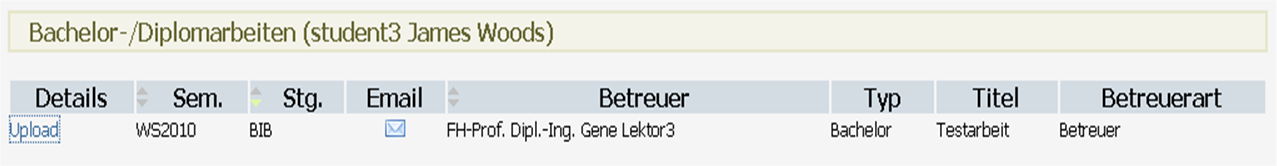
\includegraphics[width=1.0\textwidth]{abgabetool_uebersicht_student}
	\caption{�bersichtsliste der betreuten Arbeiten}
	\label{abgabetool_uebersicht_student}
\end {figure}

\subsection{Aufrufen der Termin�bersicht}
Durch einen Klick auf \textit{Upload} in der ersten Spalte der �bersichtsliste werden die Termindetails im unteren Teil der Seite angezeigt (Siehe Abbildung \ref{abgabetool_termine_student}).

\subsection{E-Mail an den/die Betreuer/Betreuerin}
Durch anklicken des Briefsymbols in der vierten Spalte wird der E-Mailclient ge�ffnet und die Empf�nger- und Absenderadresse sowie \textit{Bachelorarbeitsbetreuung} bzw. \textit{Diplomarbeitsbetreuung} als Betreff werden vorausgef�llt.

\subsection{Aufruf der Anleitung}
Rechts neben der �berschrift \textit{Bachelor- /Diplomarbeitsbetreuungen} befindet sich ein blauer Icon mit einem weissen i. Durch einfaches Klicken darauf kann diese Anleitung als pdf-Datei aufgerufen werden.

\section{Termin�bersicht}

\begin {figure}
	\centering
	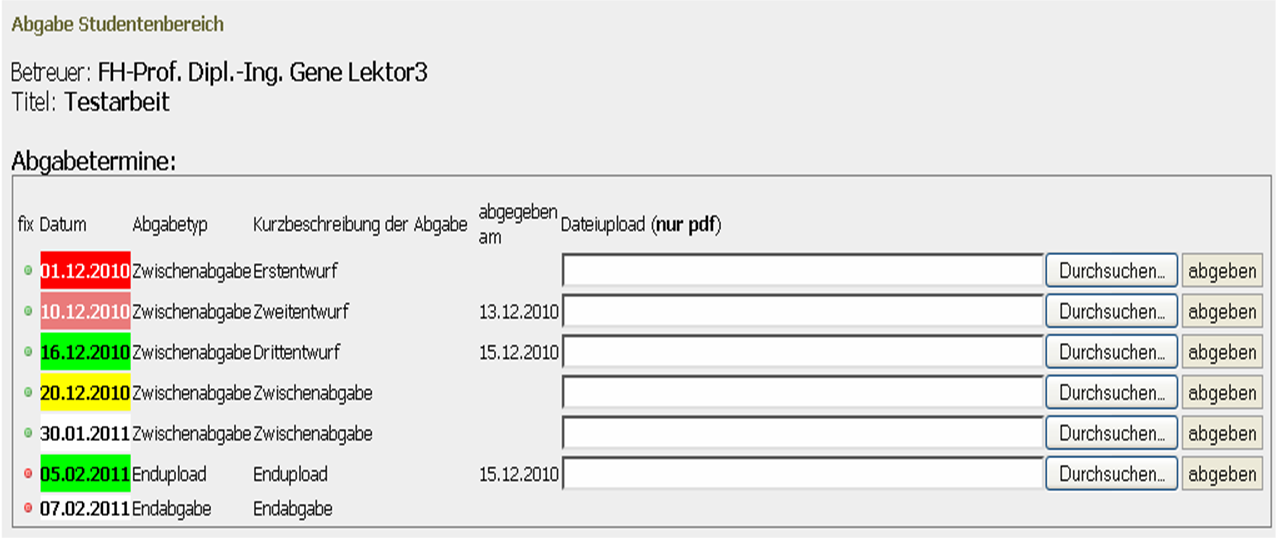
\includegraphics[width=1.0\textwidth]{abgabetool_termine_student}
	\caption{�bersicht der Termine}
	\label{abgabetool_termine_student}
\end {figure}

\subsection{Termine und Dateiupload}

\begin{itemize}
	\item Hier werden Zeilenweise die verschiedenen Termine (Erstentwurf, Zwischenabgabe, Endupload,...) mit einer kurzen Beschreibung angezeigt. 
	\item Die Farbcodierung weist auf den Terminstatus hin (siehe Abschnitt \ref{farbcode})
	\item Klicken Sie beim jeweiligen Termin auf \textit{Durchsuchen} um Ihre Festplatte nach der gew�nschten Datei zu durchsuchen. Klicken Sie danach auf \textit{abgeben} um die Datei wegzuschicken. Ihr/e Betreuer/in wird automatisch per E-Mail �ber die erfolgte Abgabe informiert. Wenn Sie erneut eine Datei hochladen, wird die bestehende Datei �berschrieben.	
	\item Die Studiengangsassistenz kann fixe Termine vergeben, erkennbar an dem roten Bullet in der Spalte \textit{fix}. Liegt ein fixer Termin in der Vergangenheit, k�nnen Sie zu diesem nichts mehr hochladen. Soll dennoch etwas hochgeladen werden, m�ssen Sie bei der Studiengangsassistenz um eine Korrektur des Termins ansuchen.
	
	\info{Es k�nnen derzeit nur Dateien im Format PDF hochgeladen werden}
\end{itemize}

\subsection{Farbcode}
\label{farbcode}

\begin{itemize}
	\item wei�:	"normaler" Termin
	\item gelb:	Termin innerhalb der n�chsten 12 Tage
	\item rot:	Termin �berschritten
	\item gr�n:	Abgabe erfolgt
	\item hellrot: Abgabe nach Termin 
\end{itemize}

\subsection{Zusatzdaten beim Endupload}
Am Termin vom Typ \textit{Endupload} erscheint nach dem Upload ein Formular (siehe Abbildung \ref{abgabetool_zusatzdaten_student}), in dem Sie dazu aufgefordert werden, zus�tzliche Daten f�r die Publikationsdatenbank einzugeben. Diese werden ebenfalls vom Betreuer/der Betreuerin auf Vollst�ndigkeit kontrolliert.
\begin{itemize}
	\item Sprache der Arbeit: Sprache in der die Arbeit verfasst wurde
	\item Kontrollierte Schlagw�rter: Hier k�nnen mit Hilfe eines Schlagwortdienstes, kontrollierte Schlagw�rter hinzugef�gt werden. Siehe Schlagwortdienst
	\item Dt. Schlagw�rter: Schlagw�rter zur Kategorisierung der Arbeit
	\item Engl. Schlagw�rter: Englische Schlagw�rter zur Kategorisierung der Arbeit 
	\item Abstract: Abstract der Arbeit
	\item Abstract engl.: Englischer Abstract der Arbeit
	\item Seitenanzahl: Anzahl der Seiten der Arbeit
	\item Eidesstattliche Erkl�rung: Akzeptieren der Erkl�rung
\end{itemize}
\begin {figure}
	\centering
	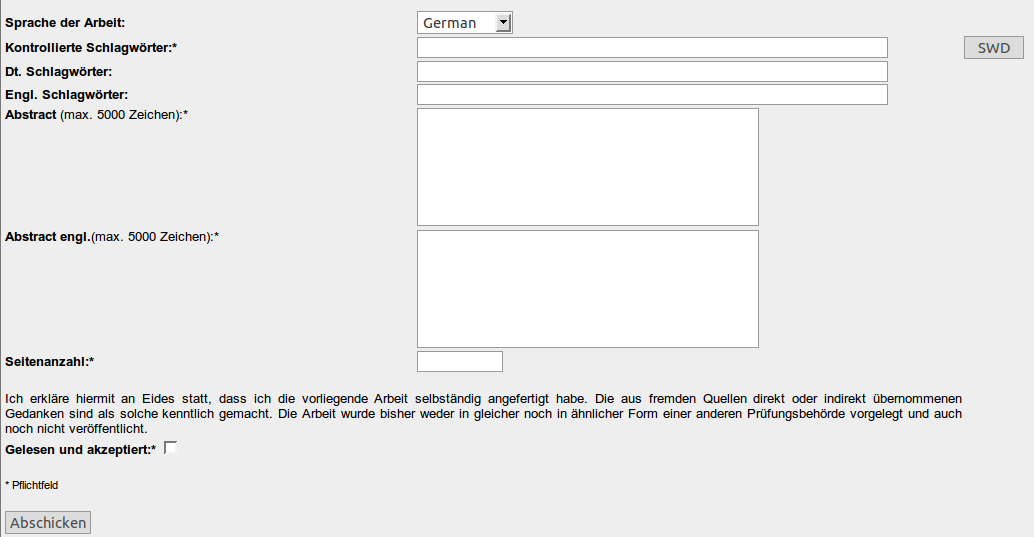
\includegraphics[width=1.0\textwidth]{abgabetool_zusatzdaten_student}
	\caption{Zusatzdaten nach dem Endupload}
	\label{abgabetool_zusatzdaten_student}
\end {figure}

\subsection{Schlagwortdienst}
Kontrollierte Schlagw�rter k�nnen mit Hilfe eines Schlagwortdienstes eingetragen werden.\\
Durch einen klick auf den Button SWD wird der Schlagwortdienst ge�ffnet. 
Sie werden auf eine externe Seite weitergeleitet.
\begin {figure}
	\centering
	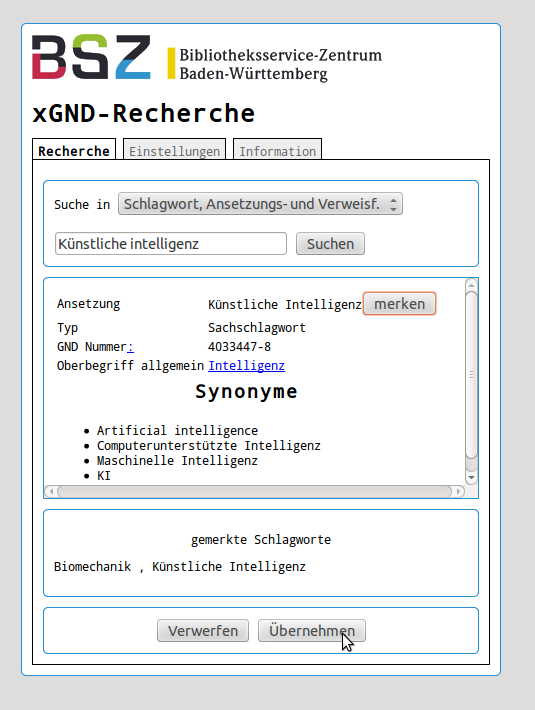
\includegraphics[width=0.5\textwidth]{abgabetool_swd}
	\caption{SWD}
	\label{SWD}
\end {figure}
\\
�ber die Suchfunktion kann nach Schlagw�rtern gesucht werden.
\\Klicken Sie auf den Button ''merken'' um Schlagw�rter auszuw�hlen.
\\Wenn Sie alle Schlagw�rter hinzugef�gt haben k�nnen Sie diese �ber den Button ''�bernehmen'' in das Abgabe-Formular �bertragen.
siehe Abbildung \ref{SWD}

\subsection{Probleme beim Upload}
Falls beim Upload der Datei Probleme auftreten kann dies folgende Gr�nde haben:

\begin{itemize}
	\item Die Dateigr��e darf maximal 15 MB betragen.
	\item Die hochzuladende Datei muss im PDF Format vorliegen. Der Upload von anderen Dateitypen ist nicht m�glich
	\item Deaktivieren Sie eventuell installierte Addons Ihres Browsers (Adblocker, NoScript, etc)
	\item Stellen Sie sicher, dass Javascript aktiviert ist
	\item Versuchen Sie die Arbeit mit einem anderen Browser hochzuladen (zB Firefox)
\end{itemize}
\chapter{Benotungstool}

\section{Quickstart}
\label{quickstart}

\subsection{Eintragen der Lehrveranstaltungsnote}

Das Benotungstool im CIS des Technikum Wien ist als Schnittstelle zwischen LektorIn und AssistentIn das zentrale Werkzeug f�r die Notenverwaltung.\\

\noindent
{\bf Bitte verwenden Sie das Tool zum Eintragen der Lehrveranstaltungsnote:}

\begin{enumerate}
\item W�hlen Sie unter \url{https://cis.technikum-wien.at} -$>$ Mein Cis -$>$ Meine LV eine Lehrveranstaltung aus. Auf der �bersichtsseite klicken Sie das Symbol 'Benotungstool' (s. Abb. \ref{uebersicht_lv}, S. \pageref{uebersicht_lv})
\item Klicken Sie nun auf im linken oberen Seitenbereich auf 'Lehrveranstaltung benoten'
\item Tragen Sie nun Noten ein und �bernehmen Sie diese mit dem '-$>$' - Knopf
(1)
\item Wenn Sie alle Noten eingetragen haben, die  Sie zu diesem Zeitpunkt
eintragen wollen (Sie k�nnen jederzeit Noten nachtragen!) k�nnen Sie diese
�ber den Knopf 'Freigabe' (im Tabellenkopf) f�r die AssistentIn freigeben.
(2)\\ 
ACHTUNG: aus Gr�nden der erh�hten Sicherheit ist bei der Freigabe der Noten
die Eingabe Ihres Passwortes erforderlich.\footnote{Es handelt sich dabei um Ihr
TW-Passwort, mit dem sie sich auch auf der CIS-Seite authentifizieren oder auf
unseren Rechnern einloggen}
\item Fertig!
\end{enumerate}


\begin{figure}[ht]
\begin{center}
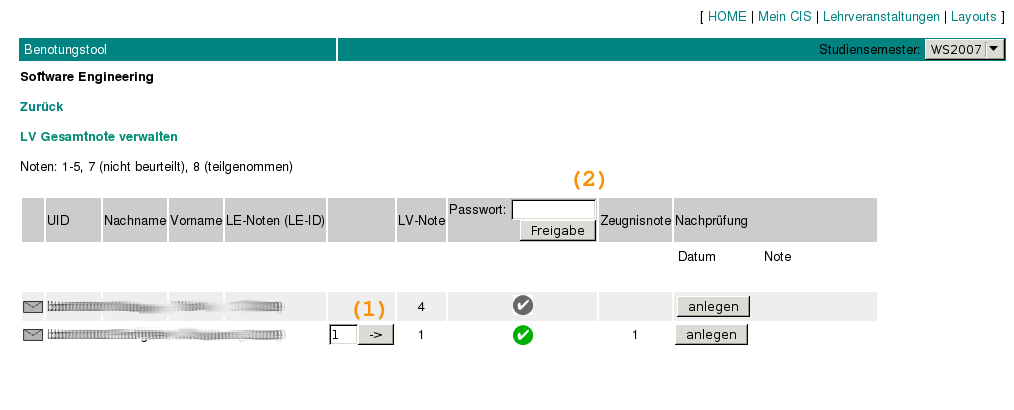
\includegraphics[width=1.0\textwidth]{benotungstool_benotung_lv.png}
\end{center}
\caption{Benotung LV}\label{benotung_lv_quick}
\end{figure}

\noindent
Weitere Informationen s. Kap. \ref{gesamtnote} auf S. \pageref{gesamtnote}\\





\section{�bungen}
\subsection{Aufbau}
\noindent
Das Anlegen der �bungen ist grunds�tzlich folgenderma�en gegliedert:
{\em �bungen} k�nnen direkt benotet werden (z. B. Tests).
Alternativ k�nnen {\em �bungen} auch beliebig viele {\em Abgaben} 
oder {\em Kreuzerllisten} enthalten. (Es ist jedoch nicht m�glich diese zu mischen).
Eine {\em Kreuzerlliste} kann dann beliebig viele Beispiele beinhalten.
(s. auch Folien im Annex S. \pageref{struktur}ff)

\subsection{�bungen anlegen und verwalten}

\begin{figure}[ht]
\begin{center}

\makebox[0pt][l]{
\includegraphics{icon_info}}%
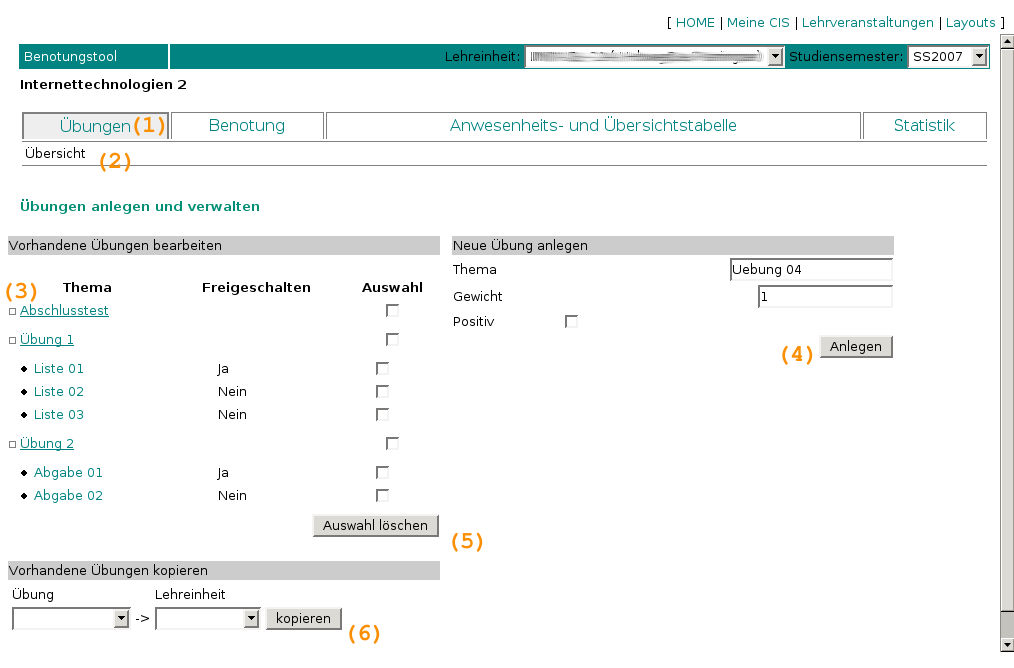
\includegraphics[width=1.0\textwidth]{benotungstool_verwaltung_01.png}

\end{center}
\caption{�bungsverwaltung - �bersicht}\label{verwaltung_01}
\end{figure}

Aktivieren Sie die Rubrik '�bungen' (s. Abb. \ref{verwaltung_01} (1)) - dies ist auch die Standard-Einstiegsseite.
In der Subnavigation (2) sehen Sie auf welcher Ebene innerhalb der �bungen Sie sich momentan befinden.

Auf der �bersichtsseite sehen Sie s�mtliche angelegten �bungen. 
Kreuzerllisten oder Abgaben innerhalb der �bungen k�nnen Sie duch klicken des kleinen Quadrats vor dem �bungsnamen anzeigen (3).

Anlegen einer neuen �bung (4): Bezeichnung und Gewicht (f�r die Notenberechnung. s. Kapitel Benotung) sind obligatorisch.
Wenn Sie das Feld 'Positiv' aktivieren, kann die errechnete Gesamtnote nur positiv sein, wenn diese �bung positiv beurteilt wurde.

L�schen von �bungen (5): Markieren Sie eine oder mehrere Eintr�ge um diese zu l�schen. Achtung: s�mtliche zugeordnete Daten werden ebenfalls gel�scht! (Untergeordnete Kreuzerllisten, Abgaben, bereits auf diese vergebene Noten, Studentenkreuzerl)

Kopieren von �bungen (6): Sie haben hier die M�glichkeit eine gesamte �bung
inkl. darunter angelegten Abgaben/Kreuzerllisten sowie s�mtlichen
Angabedateien in andere Gruppen der selben Lehrveranstaltung zu kopieren.
Einmal kopierte �bungen werden in weiterer Folge bei neuerlichem Kopieren
synchronisiert; d.h. Sie adaptieren die �bung in einer Gruppe und �bernehmen
diese dann f�r die entsprechende �bung in der anderen Gruppe.\footnote{In weiterer Folge ist auch die M�glichkeit vorgesehen �bungen aus anderen Lehrveranstaltungen und Semestern kopieren zu k�nnen}

Durch klicken eines �bungsnamens gelangen Sie zur Bearbeitungs-Ansicht der
�bung. Hier haben Sie die M�glichkeit die �bung zu editieren sowie
Untergeordnete Abgaben oder Kreuzerllisten anzulegen. Solange noch kein
untergeordnetes Element angelegt ist werden Ihnen beide angeboten. Das erste,
das Sie anlegen determiniert welcher Typus in weiterer Folge innerhalb dieser
�bung verwendet werden kann.

Sobald allerdings ein Noteneintrag zu einer �bung stattgefunden hat, k�nnen
keine untergeordneten Elemente mehr angelegt werden. (s. Kap.
\ref{benotung}, S. \pageref{benotung}) 

\subsubsection{Abgaben}

\begin{figure}[ht]
\begin{center}
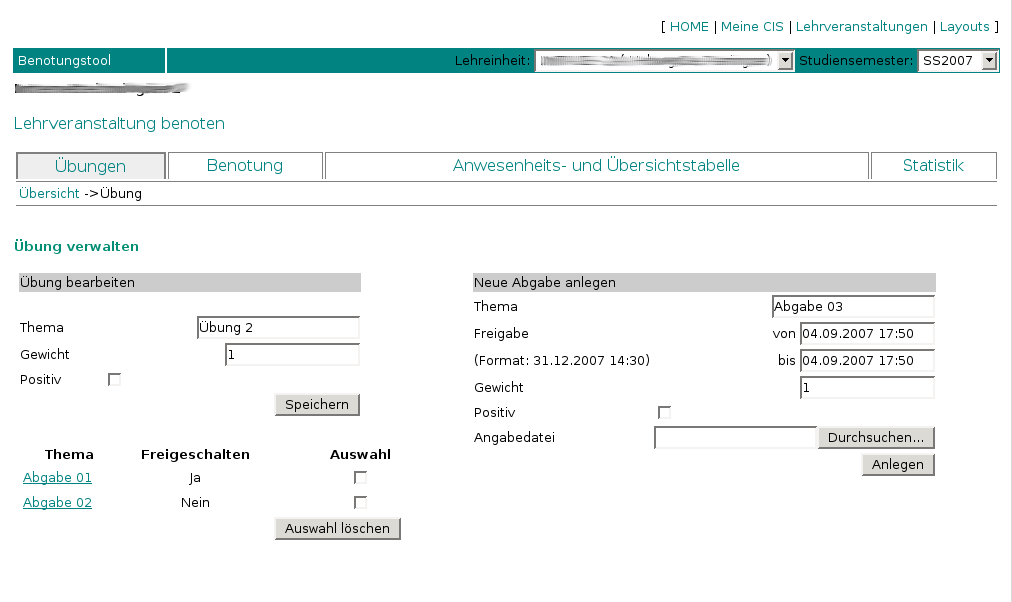
\includegraphics[width=1.0\textwidth]{benotungstool_uebung_detail_abgaben.png}
\end{center}
\caption{Abgaben anlegen}\label{uebung_detail_abgaben}
\end{figure}

Sie befinden Sich in der Bearbeitungsansicht einer �bung (s. Abb.
\ref{uebung_detail_abgaben}).

Zum Anlegen einer Abgabe definieren Sie das Thema, den Zeitraum in den Ihre
StudentInnen die M�glichkeit haben sollen die Abgabe-Datei hochzuladen, das
Gewicht die die Note auf diese Abgabe innerhalb der �bung haben soll, und ob
diese positiv sein muss. Weiters haben Sie die M�glichkeit eine Angabedatei 
hochzuladen.\footnote{Der Dateiname wird automatisch generiert und der
jeweiligen Angabe zugeordnet}

Bereits angelegte Abgaben k�nnen durch anklicken der jeweiligen Namen
bearbeitet werden. (s. Abb. \ref{abgabe_detail}). Hier k�nnen Sie Ihre
Angabedatei �ndern indem Sie sie durch eine andere �berschreiben oder l�schen
indem Sie auf den Link [del] klicken.

\begin{figure}[ht]
\begin{center}
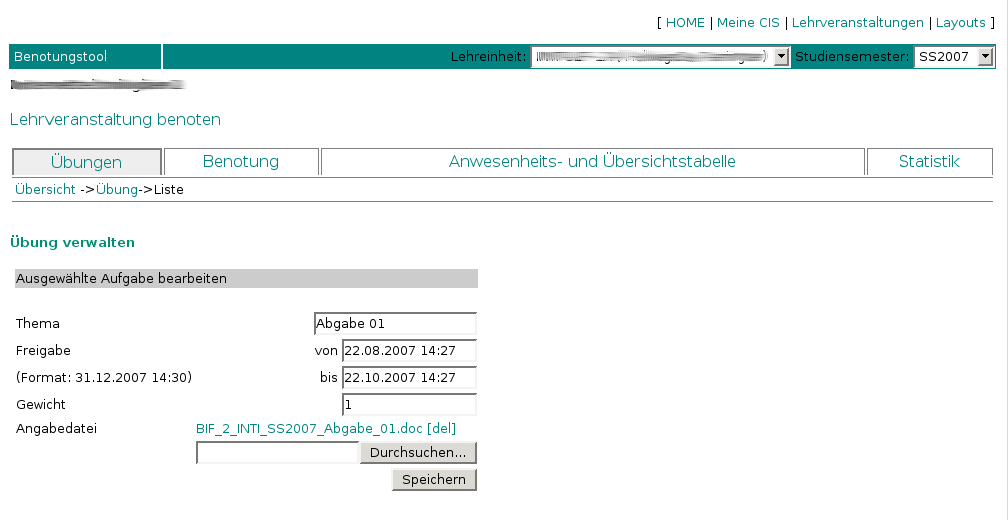
\includegraphics[width=1.0\textwidth]{benotungstool_abgabe_detail.png}
\end{center}
\caption{Abgaben bearbeiten}\label{abgabe_detail}
\end{figure}

\subsubsection{Kreuzerllisten}
\label{kap_kreuzerllisten}

Sie befinden Sich in der Bearbeitungsansicht einer �bung (s. Abb.
\ref{uebung_detail_kreuzerllisten}).

\begin{figure}[ht]
\begin{center}
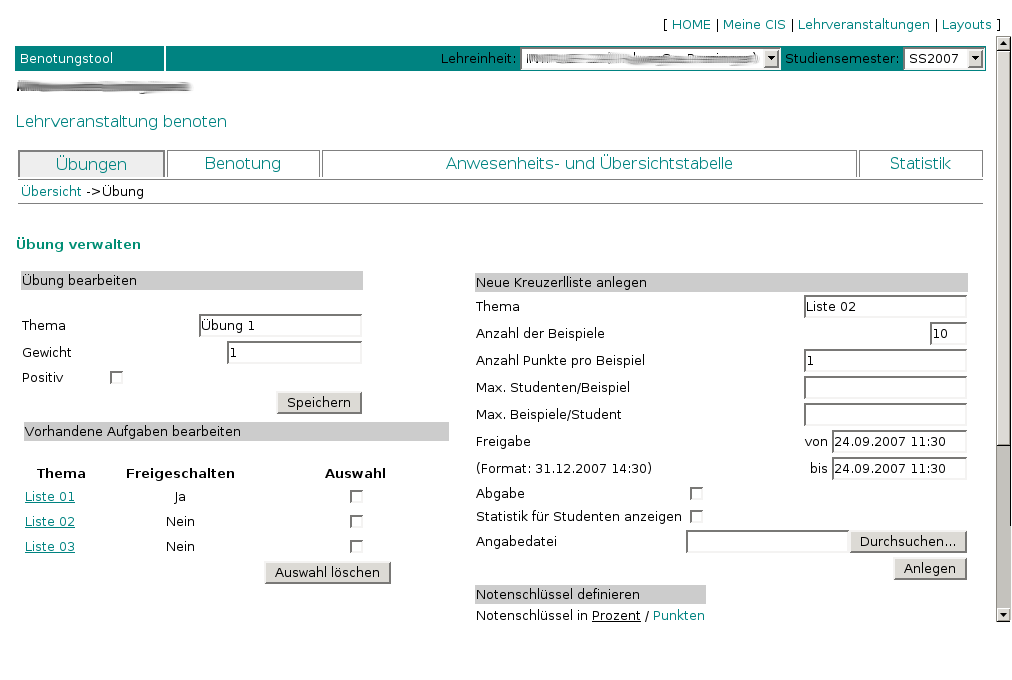
\includegraphics[width=0.9\textwidth]{benotungstool_uebung_detail_kreuzerllisten.png}
\end{center}
\caption{Kreuzerllisten anlegen}\label{uebung_detail_kreuzerllisten}
\end{figure}


Zum Anlegen einer Kreuzerlliste definieren Sie das Thema, Anzahl und
Bepunktung der Beispiele, den Zeitraum in den Ihre
StudentInnen die M�glichkeit haben sollen die Beispiele anzukreuzen, sowie ob
den StudentInnen die Statistik �ber die Verteilung der Kreuzerl angezeigt
werden soll.

Wenn Sie das Feld 'Abgabe' aktivieren, k�nnen die Studierenden eine Datei zur
Kreuzerlliste uploaden. Dies funktioniert wie bei einer Abgabe, nur dass diese
Dateien nicht gesondert von Ihnen benotet werden.

Zus�tzlich k�nnen Sie hier definieren wie viele Studenten maximal ein
bestimmtes Beispiel ankreuzen k�nnen bzw. wie viele  Beispiele maximal pro Student
angekreuzt werden k�nnen.

Weiters haben Sie die M�glichkeit eine Angabedatei zu
hochzuladen. \footnote{Der Dateiname wird automatisch generiert und der
jeweiligen Kreuzerlliste zugeordnet}


\begin{figure}[ht]
\begin{center}
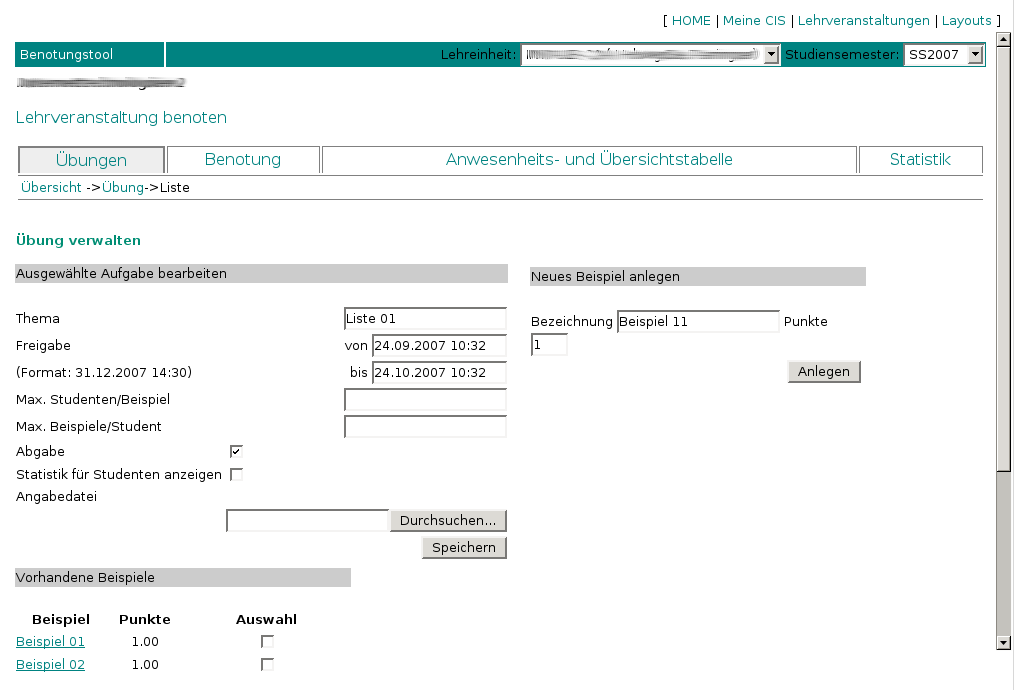
\includegraphics[width=0.9\textwidth]{benotungstool_kreuzerlliste_detail.png}
\end{center}
\caption{Kreuzerllisten bearbeiten}\label{kreuzerlliste_detail}
\end{figure}

Bereits angelegte Kreuzerllisten k�nnen durch anklicken der jeweiligen Namen
bearbeitet werden. (s. Abb. \ref{kreuzerlliste_detail}). Hier k�nnen Beispiele
hinzugef�gt, gel�scht oder durch anklicken editiert werden. Weiters k�nnen Sie
Ihre
Angabedatei �ndern indem Sie sie durch eine andere �berschreiben oder l�schen
indem Sie auf den Link [del] klicken.

\subsubsection{Notenschl�ssel}
\label{kap_notenschluessel}
Mithilfe des Notenschl�ssels werden die Punkte s�mtlicher Beispiele s�mtlicher
Kreuzerllisten innerhalb EINER �bung zu einer Note umgerechnet.
Der Notenschl�ssel wird auf Ebene jener �bung definiert, die die Kreuzerllisten
enth�lt. 

Solange noch kein Notenschl�ssel angelegt ist, werden die
Kreuzerllisten dieser �bung nicht in die automatisch errechnete Gesamtnote
einbezogen.

Sie haben die M�glichkeit den Notenschl�ssel in {\em Prozent} oder in {\em
Punkten} zu definieren (s. Abb. \ref{notenschluessel})

\begin{figure}[ht]
\begin{center}
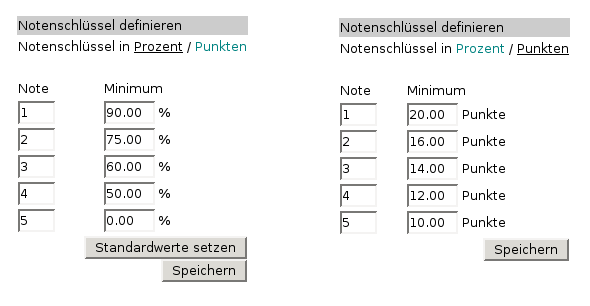
\includegraphics[width=0.8\textwidth]{benotungstool_notenschluessel.png}
\caption{Notenschl�ssel in Prozent oder Punkten}\label{notenschluessel}
\end{center}
\end{figure}

Schalten Sie zwischen diesen beiden Modi um, indem Sie auf den jeweiligen Link
klicken. Der \underline{unterstrichene Modus} ist aktiv.

Beim {\em Prozent}-Modus haben Sie die M�glichkeit durch den Knopf
'Standardwerte setzen' die Felder mit solchen vorauszuf�llen.
Adaptieren Sie diese gegebenenfalls und vergessen Sie nicht zu speichern.

\section{Benotung}
\label{benotung}
Aktivieren Sie die Rubrik Benotung (s. Abb. \ref{benotung_uebungen} (1))

\subsection{�bersicht und Benotung der �bungen}
\label{ben}

\begin{figure}[ht]
\begin{center}
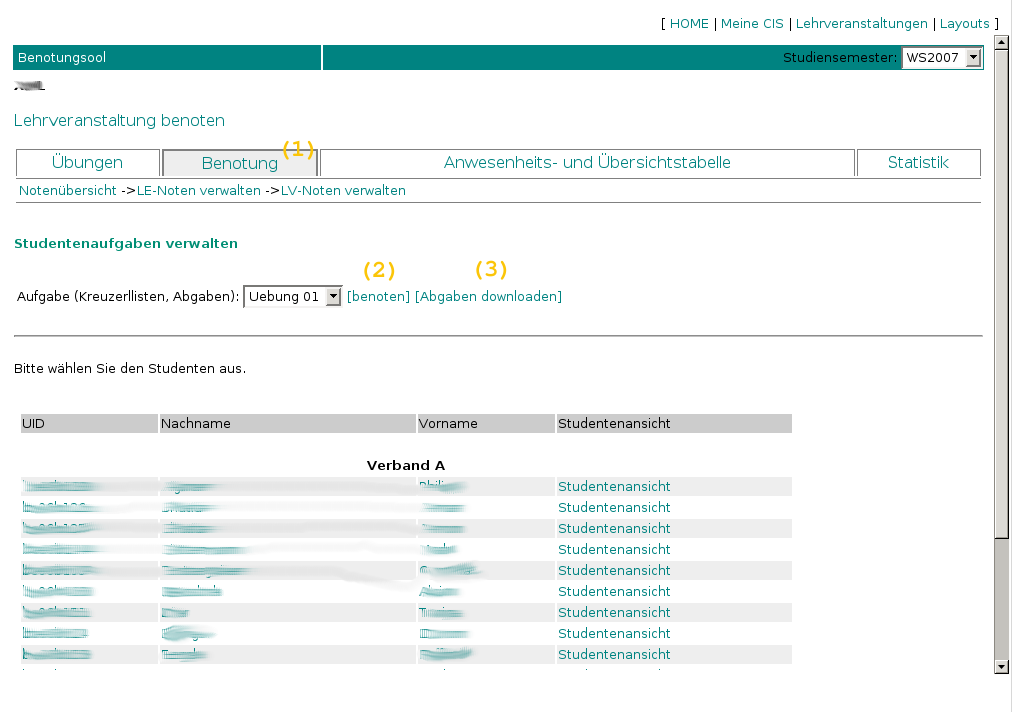
\includegraphics[width=1.0\textwidth]{benotungstool_benotung.png}
\end{center}
\caption{Benotung �bungen}\label{benotung_uebungen}
\end{figure}

W�hlen Sie eine �bung, Abgabe oder Kreuzerlliste im Dropdown-Men� aus und
klicken Sie 'benoten'(s. Abb \ref{benotung_uebungen} (2)).
Es �ffnet sich eine neue Seite mit der Liste aller
StudentInnen und einem Notenfeld oder Checkboxen f�r die Beispiele einer
Kreuzerlliste, sowie der Abgabedatei der StudentIn (s. Abb.
\ref{notenliste}).
Nehmen Sie Ihre Eintr�ge vor und speichern Sie die Seite mit
dem Knopf rechts unten ab. Schlie�en Sie die Seite.

\begin{figure}[ht]
\begin{center}
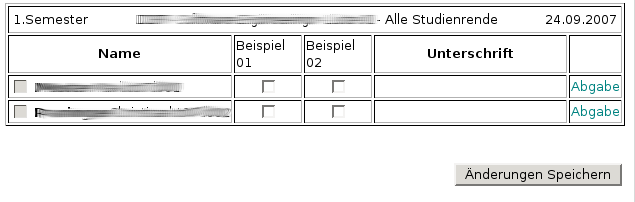
\includegraphics[width=0.7\textwidth]{benotungstool_notenliste.png}
\end{center}
\caption{Notenliste}\label{notenliste}
\end{figure}


Wenn zu einer Abgabe Studentendateien vorliegen, so wird neben dem Link
'benoten' ein weiterer Link zum Download einer ZIP-Datei mit allen Studentendateien 
dieser Abgabe aktiv (3).

Klicken Sie auf den Namen einer StudentIn, so k�nnen Sie f�r diese im Detail
Noten, Kreuzerl, Mitarbeitspunkte und Anmerkungen vergeben.\footnote{Im
Wesentlichen ist hier die Struktur des alten 'Kreuzerl-Tools erhalten geblieben'}

\subsection{Studentenansicht}
\label{studentenansicht}
F�r die Studenten in Ihrer Gruppe k�nnen Sie durch klicken auf den Link
'Studentenansicht' (rechts neben den Namen in der Liste) in einem neuen
Fenster die Ansicht des jeweiligen Studenten anzeigen lassen. In
diesem Fesnter nehmen Sie die Idetit�t der StudentIn an, k�nnen dort alle
Funktionen so bedienen wie es auch die StudentIn kann. 

Diese Funktion ist allerdings nur f�r Sie zu �bersichts-/Demonstrationszwecken
gedacht. Verwenden Sie zum �ndern der Daten (Kreuzerl hinzuf�gen/l�schen) immer
das Lektoren-Admin-Interface wie unter Punkt \ref{ben} beschrieben!

\subsection{LE-Noten verwalten}
\begin{figure}[ht]
\begin{center}
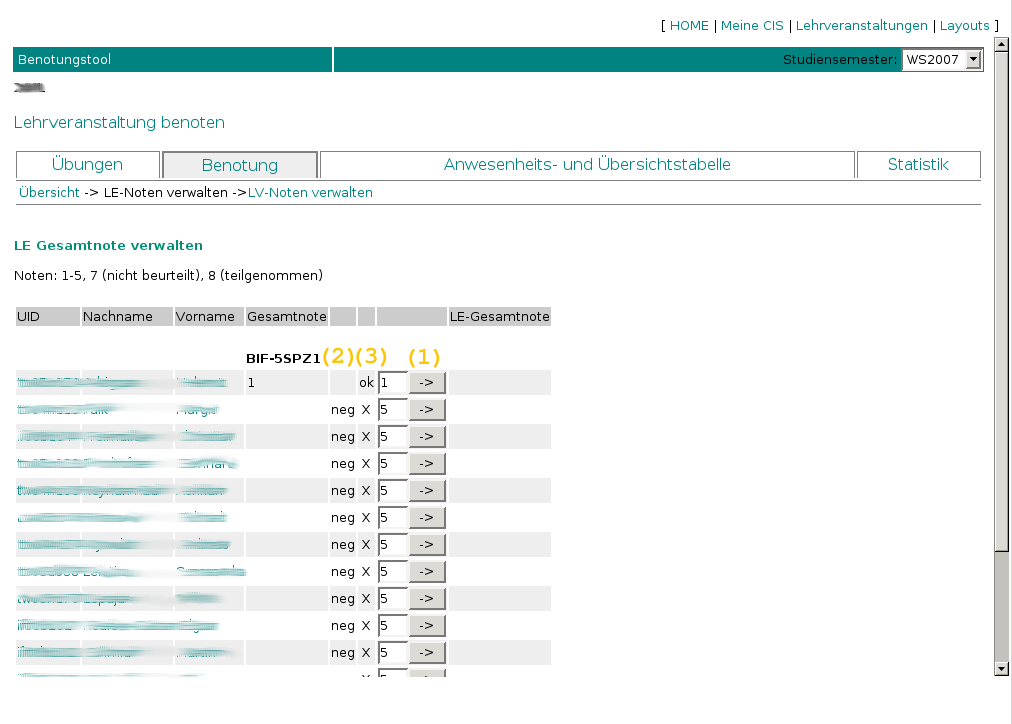
\includegraphics[width=1.0\textwidth]{benotungstool_benotung_le.png}
\end{center}
\caption{Benotung Lehreinheit}\label{benotung_le}
\end{figure}

Aus den Noten der einzelnen �bungen, Abgaben und Kreuzerllisten wird �ber die
von Ihnen definierte Gewichtung bzw. im Falle der Kreuzerllisten den
Notenschl�ssel eine Gesamtnote f�r die Lehreinheit errechnet.
Diese wird Ihnen gerundet zur �bernahme als LE-Gesamtnote vorgeschlagen.
�berpr�fen/korrigieren Sie diese und �bernehmen Sie sie mittels '-$>$' - Knopf.
(s. Abb. \ref{benotung_le} (1))

Weitere Felder:
'neg' (2) in der Spalte neben der errechneten Note bedeutet, dass zumindest als zwingend positiv
definierte Note negativ ist; 'ok'/'x' (3) zeigt an, ob alle Teilnoten verf�gbar sind.

%\section{Gesamtnote}
\label{gesamtnote}
W�hlen Sie unter \url{https://cis.technikum-wien.at} -$>$ Mein Cis -$>$ Meine LV eine Lehrveranstaltung aus. Auf der �bersichtsseite klicken Sie das Symbol 'Gesamtnote' um zur Benotungsseite zu gelangen.

\subsection{Eintragen der Note}
\subsubsection{Manuelle Eintragung der Gesamtnote}
\label{ben}

\begin{enumerate}
\item Tragen Sie die Noten ein (1) und �bernehmen Sie diese mit dem '-$>$' - Knopf
\item Nachdem Sie alle Noten eingetragen haben, k�nnen Sie diese Freigeben siehe Kap. \ref{freigabe} auf S. \pageref{freigabe}\\
\end{enumerate}

\begin{figure}[ht]
\begin{center}
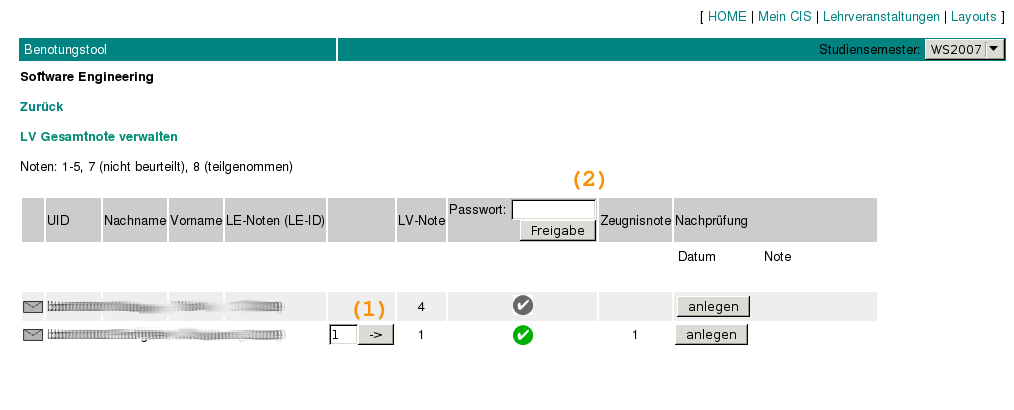
\includegraphics[width=1.0\textwidth]{benotungstool_benotung_lv.png}
\end{center}
\caption{Benotung Lehrveranstaltung}\label{benotung_lv}
\end{figure}

\subsubsection{Noten aus �bungstool (Kreuzerltool) �bernehmen}
\label{ben}

Wenn eine �bung im �bungstool (Kreuzerltool) angelegt und benotet wurde, scheint die Note in der Gesamtbeurteilung auf.
Wenn mehrere Lehreinheiten zu dieser Lehrveranstaltung vorhanden sind, wird das mittel aller Noten als Gesamtnote vorgeschlagen.

Die Notenfelder sind bereits vorausgef�llt. �bernehmen Sie diese mit dem '-$>$' - Knopf.

\subsubsection{Noten aus Moodle �bernehmen}
\label{ben}

Wenn ein Moodle-Kurs angelegt und benotet wurde, scheint die Note automatisch in der Gesamtbeurteilung auf.
Wenn mehrere Kurse zu dieser Lehrveranstaltung vorhanden sind, wird das Mittel aller Noten als Gesamtnote vorgeschlagen.
Die Notenfelder sind bereits vorausgef�llt. �bernehmen Sie diese mit dem '-$>$' - Knopf.

\subsubsection{Notenimport aus Excel}
\label{ben}

Es besteht die M�glichkeit, Noten aus einem Excel-File zu importieren. Folgende Schritte sind dazu n�tig:

\begin{enumerate}
\item Laden Sie sich die Excel-Notenliste unter CIS -$>$ Lehrveranstaltungen -$>$ Anwesenheits- und Notenlisten -$>$ Notenliste herunter
\item Tragen Sie im Excel-File die Noten ein
\item Markieren Sie im Excel die beiden Spalten Matrikelnummer und Note f�r jene Studenten f�r die Sie die Noten importieren m�chten. (ohne �berschrift)
\begin{figure}[ht]
\begin{center}
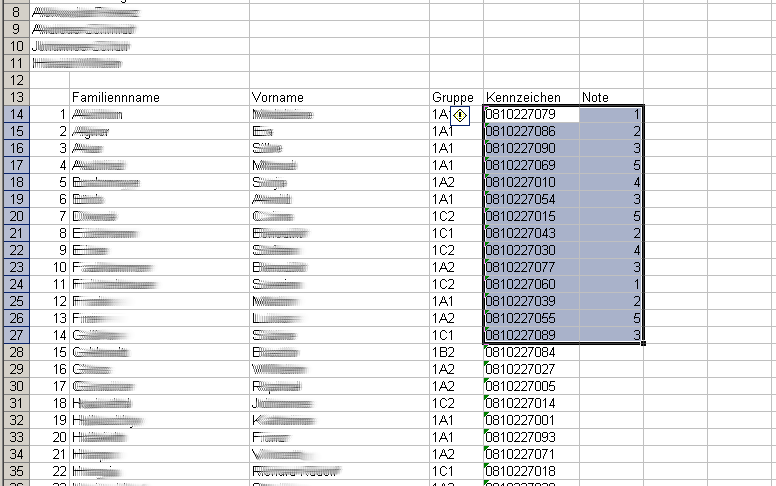
\includegraphics[width=1.0\textwidth]{CIS_Gesamtnote_Excelimport.png}
\end{center}
\caption{Excelimport}\label{excelimport}
\end{figure}
\item Kopieren Sie die markierten Spalten mittels $<$strg$>$+$<$c$>$ oder Bearbeiten-$>$Kopieren in die Zwischenablage
\item Mit einem Klick auf den Knopf 'Import' werden die Noten �bernommen.
\end{enumerate}
\achtung {Bestehende Noten werden ohne Nachfrage �berschrieben}
Damit der Notenimport funktioniert m�ssen im Browser einige Sicherheitseinstellungen vorgenommen werden:

\begin{enumerate}
\item Firefox / Mozilla
	\begin{enumerate}
	\item �ffnen Sie ein neues Browserfenster
	\item geben sie 'about:config' in die Adressleiste ein. 
	(M�glicherweise erscheint hier eine Warnmeldung die Sie mit einem klick auf den angezeigten Knopf �berspringen)
	\item Suchen sie den Eintrag 'signed.applets.codebase\_principal\_support'
	\item mit einem Doppelklick muss diese Einstellung auf 'true' gesetzt werden
	\end{enumerate}
	\achtung {Durch die Aktivierung dieses Eintrages wird ein Sicherheitsloch ge�ffnet. Wir empfehlen daher diese Einstellung nach dem
	Import wieder zur�ckzusetzen.}
\item InternetExplorer
	\begin{enumerate}
	\item Beim IE m�ssen keine Einstellungen vorgenommen werden. Wenn auf 'Import' geklickt wird erscheint (bei IE7) eine Warnungmeldung die sie mit 'Zugriff zulassen' best�tigen m�ssen.
	\end{enumerate}
\item Safari, Opera
	\begin{enumerate}
	\item Mit den Browsern Safari und Opera kann der Notenimport NICHT verwendet werden. Bitte verwenden Sie Firefox oder den InternetExplorer
	\end{enumerate}
\end{enumerate}

\subsection{Freigabe der Noten}
\label{freigabe}

Wenn Sie alle Noten eingetragen haben, die  Sie zu diesem Zeitpunkt
eintragen wollen (Sie k�nnen jederzeit Noten nachtragen!) k�nnen Sie diese
�ber den Knopf 'Freigabe' (im Tabellenkopf) f�r die AssistentIn freigeben.
(2)

\info {
ACHTUNG!! aus Gr�nden der erh�hten Sicherheit ist bei der Freigabe der Noten
die Eingabe Ihres Passwortes erforderlich.\footnote{Es handelt sich dabei um Ihr
TW-Passwort, mit dem sie sich auch auf der CIS-Seite authentifizieren oder auf
unseren Rechnern einloggen}
}

\begin{itemize}
	\item Zul�ssige Noten: 1-5, 7 (nicht beurteilt), 8 (teilgenommen)
	\item Bei der Freigabe wird ein Info-Email an Sie und die zust�ndige
	Studiengangs\-assistentIn geschickt. Enthalten sind Mat. Nr., Vorname,
	Nachname und Note der neuen oder ge�nderten Eintr�ge.
	\item Freigegebene Eintr�ge sind mit einem gr�nen Kreis mit H�kchen gekennzeichnet.
	\item Wenn Sie bereits freigegebene Noten ver�ndern, werden diese mit einem grauen Kreis mit H�kchen markiert (als Hinweis f�r Sie, dass die AssistentIn dar�ber noch nicht per Mail informiert wurde. Sie sieht allerdings diese neue Note sofort in ihrer Oberfl�che)
	\item Die freigegebenen Noten kann die AssistentIn nun als Zeugnisnote �bernehmen, die dann im n�chsten Feld f�r Sie zur Kontrolle angezeigt wird.
	\item Wenn sich die Zeugnisnote von der von Ihnen freigegebenen Note unterscheidet wird erstere rot umrandet markiert.
\end{itemize}

\subsection{Eintragen einer Nachpr�fung (2. Termin)}
\label{nachpruefung}

Sobald Sie eine LV-Note eingetragen und haben erscheint (bei Neuladen der
Seite, etwa durch die Freigabe der Noten) rechts neben der Zeugnisnote ein
Knopf zum Anlegen einer Nachpr�fung. Sobald eine solche angelegt ist sehen Sie
Datum und Note, sowie einen Editier-Knopf (s. Abb.
\ref{benotung_lv_nachpruefung_quick} (1),(2)).

\begin{figure}[ht]
\begin{center}
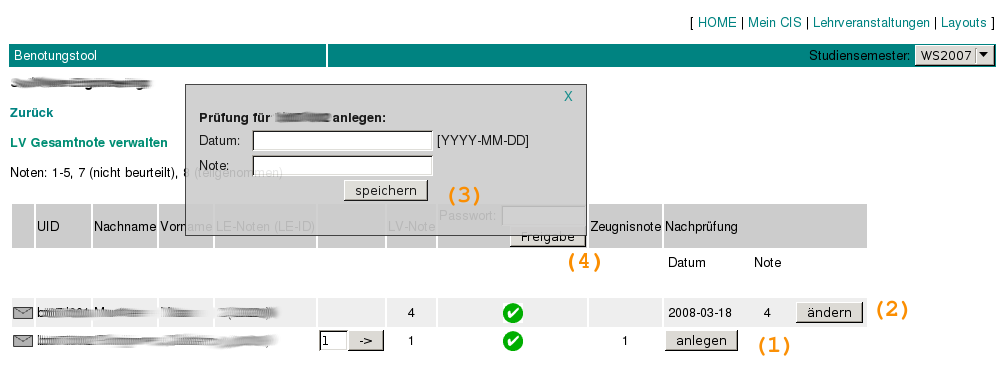
\includegraphics[width=1.0\textwidth]{benotungstool_benotung_lv_nachpruefung.png}
\end{center}
\caption{Benotung LV Nachpr�fung}\label{benotung_lv_nachpruefung_quick}
\end{figure}

Klicken Sie auf den jeweiligen Button, um eine Nachpr�fung anzulegen oder zu
editieren. Es �ffnet sich eine Eingabemaske (3) wo Sie Datum und Note eingeben und
mit Klick auf den 'speichern'-Knopf �bernehmen.

\begin{itemize}
    \item Beachten Sie bei der Einagbe bitte das Datumsformat: JJJJ-MM-DD
    \item Als Notenwerte sind wieder 1-5, 7 (nicht beurteilt), 8
    (teilgenommen) und hier zus�tzlich 9 (noch nicht eingetragen) zul�ssig. 
    Wenn Sie das Notenfeld leer lassen, wird dies als 9 interpretiert.
    \item Vergessen Sie nicht nach dem Eintragen neuer Noten diese erneut
    mithilfe des Buttons 'Freigabe' freizugeben (4).
\end{itemize}

%\newpage



\section{Anwesenheits- und �bersichtstabelle}

Dieser Bereich ist noch im Aufbau. Die Momentanen Tabellen sind im Wesentlichen
jene der alten 'Kreuzerl-Tool'-Implementierung

\section{Gesamtnote}
\label{gesamtnote}
W�hlen Sie unter \url{https://cis.technikum-wien.at} -$>$ Mein Cis -$>$ Meine LV eine Lehrveranstaltung aus. Auf der �bersichtsseite klicken Sie das Symbol 'Gesamtnote' um zur Benotungsseite zu gelangen.

\subsection{Eintragen der Note}
\subsubsection{Manuelle Eintragung der Gesamtnote}
\label{ben}

\begin{enumerate}
\item Tragen Sie die Noten ein (1) und �bernehmen Sie diese mit dem '-$>$' - Knopf
\item Nachdem Sie alle Noten eingetragen haben, k�nnen Sie diese Freigeben siehe Kap. \ref{freigabe} auf S. \pageref{freigabe}\\
\end{enumerate}

\begin{figure}[ht]
\begin{center}
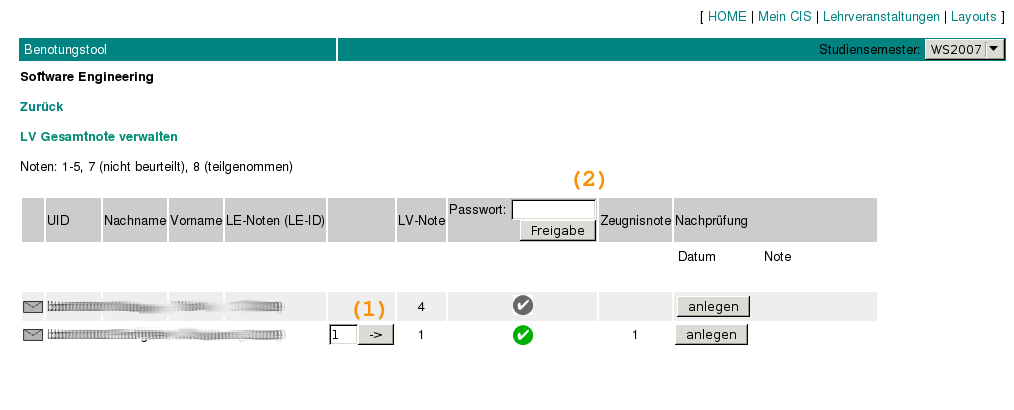
\includegraphics[width=1.0\textwidth]{benotungstool_benotung_lv.png}
\end{center}
\caption{Benotung Lehrveranstaltung}\label{benotung_lv}
\end{figure}

\subsubsection{Noten aus �bungstool (Kreuzerltool) �bernehmen}
\label{ben}

Wenn eine �bung im �bungstool (Kreuzerltool) angelegt und benotet wurde, scheint die Note in der Gesamtbeurteilung auf.
Wenn mehrere Lehreinheiten zu dieser Lehrveranstaltung vorhanden sind, wird das mittel aller Noten als Gesamtnote vorgeschlagen.

Die Notenfelder sind bereits vorausgef�llt. �bernehmen Sie diese mit dem '-$>$' - Knopf.

\subsubsection{Noten aus Moodle �bernehmen}
\label{ben}

Wenn ein Moodle-Kurs angelegt und benotet wurde, scheint die Note automatisch in der Gesamtbeurteilung auf.
Wenn mehrere Kurse zu dieser Lehrveranstaltung vorhanden sind, wird das Mittel aller Noten als Gesamtnote vorgeschlagen.
Die Notenfelder sind bereits vorausgef�llt. �bernehmen Sie diese mit dem '-$>$' - Knopf.

\subsubsection{Notenimport aus Excel}
\label{ben}

Es besteht die M�glichkeit, Noten aus einem Excel-File zu importieren. Folgende Schritte sind dazu n�tig:

\begin{enumerate}
\item Laden Sie sich die Excel-Notenliste unter CIS -$>$ Lehrveranstaltungen -$>$ Anwesenheits- und Notenlisten -$>$ Notenliste herunter
\item Tragen Sie im Excel-File die Noten ein
\item Markieren Sie im Excel die beiden Spalten Matrikelnummer und Note f�r jene Studenten f�r die Sie die Noten importieren m�chten. (ohne �berschrift)
\begin{figure}[ht]
\begin{center}
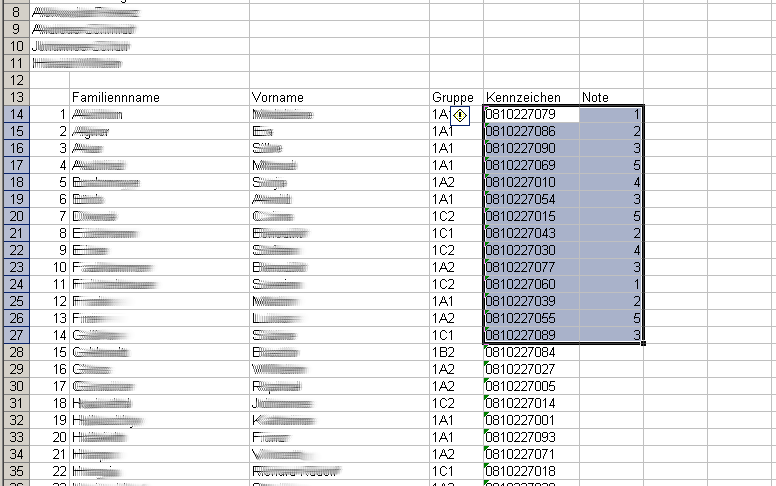
\includegraphics[width=1.0\textwidth]{CIS_Gesamtnote_Excelimport.png}
\end{center}
\caption{Excelimport}\label{excelimport}
\end{figure}
\item Kopieren Sie die markierten Spalten mittels $<$strg$>$+$<$c$>$ oder Bearbeiten-$>$Kopieren in die Zwischenablage
\item Mit einem Klick auf den Knopf 'Import' werden die Noten �bernommen.
\end{enumerate}
\achtung {Bestehende Noten werden ohne Nachfrage �berschrieben}
Damit der Notenimport funktioniert m�ssen im Browser einige Sicherheitseinstellungen vorgenommen werden:

\begin{enumerate}
\item Firefox / Mozilla
	\begin{enumerate}
	\item �ffnen Sie ein neues Browserfenster
	\item geben sie 'about:config' in die Adressleiste ein. 
	(M�glicherweise erscheint hier eine Warnmeldung die Sie mit einem klick auf den angezeigten Knopf �berspringen)
	\item Suchen sie den Eintrag 'signed.applets.codebase\_principal\_support'
	\item mit einem Doppelklick muss diese Einstellung auf 'true' gesetzt werden
	\end{enumerate}
	\achtung {Durch die Aktivierung dieses Eintrages wird ein Sicherheitsloch ge�ffnet. Wir empfehlen daher diese Einstellung nach dem
	Import wieder zur�ckzusetzen.}
\item InternetExplorer
	\begin{enumerate}
	\item Beim IE m�ssen keine Einstellungen vorgenommen werden. Wenn auf 'Import' geklickt wird erscheint (bei IE7) eine Warnungmeldung die sie mit 'Zugriff zulassen' best�tigen m�ssen.
	\end{enumerate}
\item Safari, Opera
	\begin{enumerate}
	\item Mit den Browsern Safari und Opera kann der Notenimport NICHT verwendet werden. Bitte verwenden Sie Firefox oder den InternetExplorer
	\end{enumerate}
\end{enumerate}

\subsection{Freigabe der Noten}
\label{freigabe}

Wenn Sie alle Noten eingetragen haben, die  Sie zu diesem Zeitpunkt
eintragen wollen (Sie k�nnen jederzeit Noten nachtragen!) k�nnen Sie diese
�ber den Knopf 'Freigabe' (im Tabellenkopf) f�r die AssistentIn freigeben.
(2)

\info {
ACHTUNG!! aus Gr�nden der erh�hten Sicherheit ist bei der Freigabe der Noten
die Eingabe Ihres Passwortes erforderlich.\footnote{Es handelt sich dabei um Ihr
TW-Passwort, mit dem sie sich auch auf der CIS-Seite authentifizieren oder auf
unseren Rechnern einloggen}
}

\begin{itemize}
	\item Zul�ssige Noten: 1-5, 7 (nicht beurteilt), 8 (teilgenommen)
	\item Bei der Freigabe wird ein Info-Email an Sie und die zust�ndige
	Studiengangs\-assistentIn geschickt. Enthalten sind Mat. Nr., Vorname,
	Nachname und Note der neuen oder ge�nderten Eintr�ge.
	\item Freigegebene Eintr�ge sind mit einem gr�nen Kreis mit H�kchen gekennzeichnet.
	\item Wenn Sie bereits freigegebene Noten ver�ndern, werden diese mit einem grauen Kreis mit H�kchen markiert (als Hinweis f�r Sie, dass die AssistentIn dar�ber noch nicht per Mail informiert wurde. Sie sieht allerdings diese neue Note sofort in ihrer Oberfl�che)
	\item Die freigegebenen Noten kann die AssistentIn nun als Zeugnisnote �bernehmen, die dann im n�chsten Feld f�r Sie zur Kontrolle angezeigt wird.
	\item Wenn sich die Zeugnisnote von der von Ihnen freigegebenen Note unterscheidet wird erstere rot umrandet markiert.
\end{itemize}

\subsection{Eintragen einer Nachpr�fung (2. Termin)}
\label{nachpruefung}

Sobald Sie eine LV-Note eingetragen und haben erscheint (bei Neuladen der
Seite, etwa durch die Freigabe der Noten) rechts neben der Zeugnisnote ein
Knopf zum Anlegen einer Nachpr�fung. Sobald eine solche angelegt ist sehen Sie
Datum und Note, sowie einen Editier-Knopf (s. Abb.
\ref{benotung_lv_nachpruefung_quick} (1),(2)).

\begin{figure}[ht]
\begin{center}
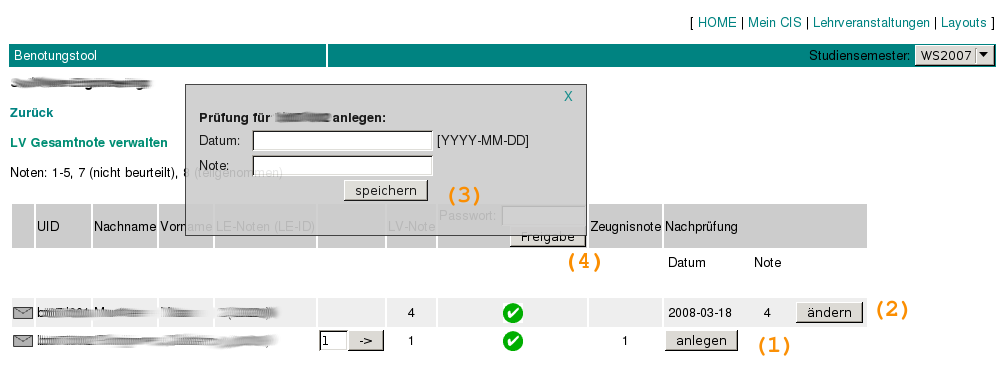
\includegraphics[width=1.0\textwidth]{benotungstool_benotung_lv_nachpruefung.png}
\end{center}
\caption{Benotung LV Nachpr�fung}\label{benotung_lv_nachpruefung_quick}
\end{figure}

Klicken Sie auf den jeweiligen Button, um eine Nachpr�fung anzulegen oder zu
editieren. Es �ffnet sich eine Eingabemaske (3) wo Sie Datum und Note eingeben und
mit Klick auf den 'speichern'-Knopf �bernehmen.

\begin{itemize}
    \item Beachten Sie bei der Einagbe bitte das Datumsformat: JJJJ-MM-DD
    \item Als Notenwerte sind wieder 1-5, 7 (nicht beurteilt), 8
    (teilgenommen) und hier zus�tzlich 9 (noch nicht eingetragen) zul�ssig. 
    Wenn Sie das Notenfeld leer lassen, wird dies als 9 interpretiert.
    \item Vergessen Sie nicht nach dem Eintragen neuer Noten diese erneut
    mithilfe des Buttons 'Freigabe' freizugeben (4).
\end{itemize}

\section{Statistik}

In diesem Bereich werden Statistiken �ber die eingetragenen Kreuzerl der
einzelnen Kreuzerllisten angezeigt, wie sie auch die Studenten sehen, wenn Sie
bei einer Kreuzerlliste die Box 'Statistik' markiert haben.


\section{Annex}

Hier finden Sie das Benotungstool:

\url{https://cis.technikum-wien.at} -$>$ Mein Cis -$>$ Meine LV
klicken Sie eine Lehrveranstaltung an um auf deren �bersichtsseite zu
gelangen. Dort finden Sie den Link zum Benotungstool.
\begin{figure}[ht]
\begin{center}
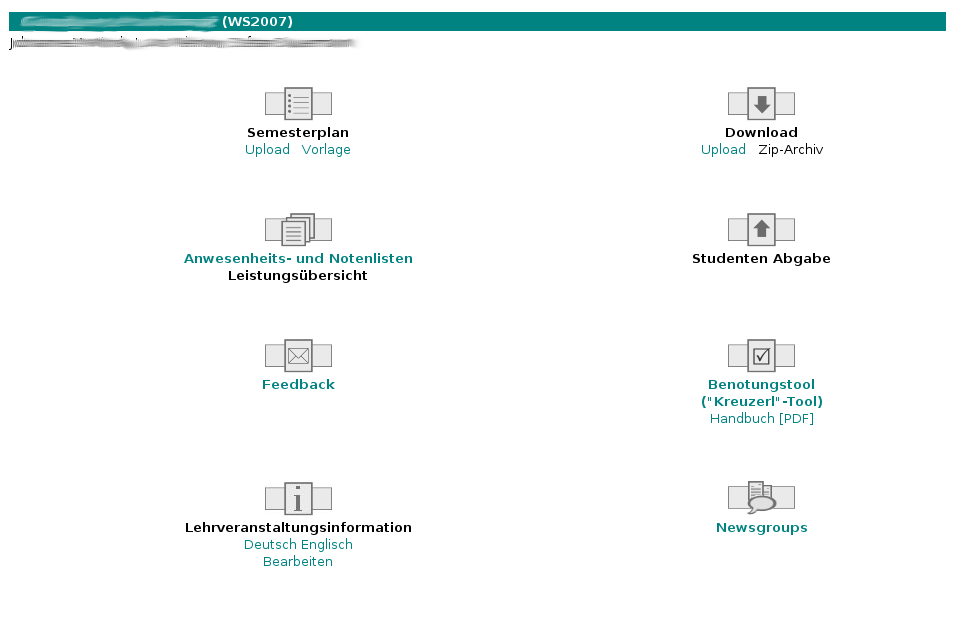
\includegraphics[width=1.0\textwidth]{benotungstool_uebersicht_lv.png}
\end{center}
\caption{�bersicht LV}\label{uebersicht_lv}
\end{figure}

\begin{figure}[ht]
\begin{center}
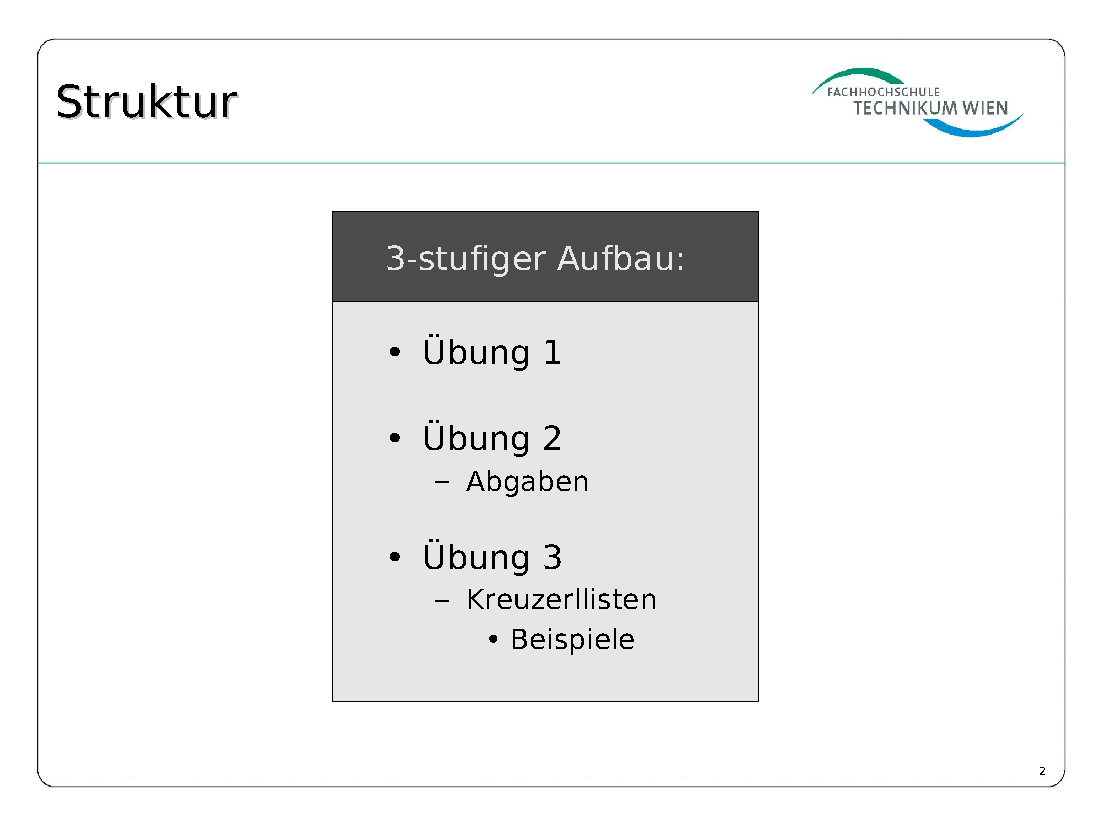
\includegraphics[width=0.9\textwidth]{benotungstool_praes_01.png}
\end{center}
\caption{Pr�sentation: Struktur}\label{struktur}
\end{figure}

\begin{figure}[ht]
\begin{center}
\includegraphics[width=0.9\textwidth]{benotungstool_praes_02.png}
\end{center}
\caption{Pr�sentation: �bung}\label{uebung}
\end{figure}

\begin{figure}[ht]
\begin{center}
\includegraphics[width=0.9\textwidth]{benotungstool_praes_03.png}
\end{center}
\caption{Pr�sentation: �bung mit Abgaben}\label{uebung_abgabe}
\end{figure}

\begin{figure}[ht]
\begin{center}
\includegraphics[width=0.9\textwidth]{benotungstool_praes_04.png}
\end{center}
\caption{Pr�sentation: �bung mit Kreuzerllisten}\label{uebung_kreuzerllisten}
\end{figure}




%% Kapitel Ende   %%%%%%%%%%%%%%%%%%%%%%%%%%%%%%%%%%%%%%%%%%%%%%%%%
\appendix							% Beginn des Anhangs
%%\chapter{Schluss}
%\listoftables					% Tabellenverzeichnis
%\listoffigures				% Abbildungsverzeichnis
\end{document}
